\noindent\begin{figure}[htb]
\centering
\begin{minipage}[t]{0.48\textwidth}
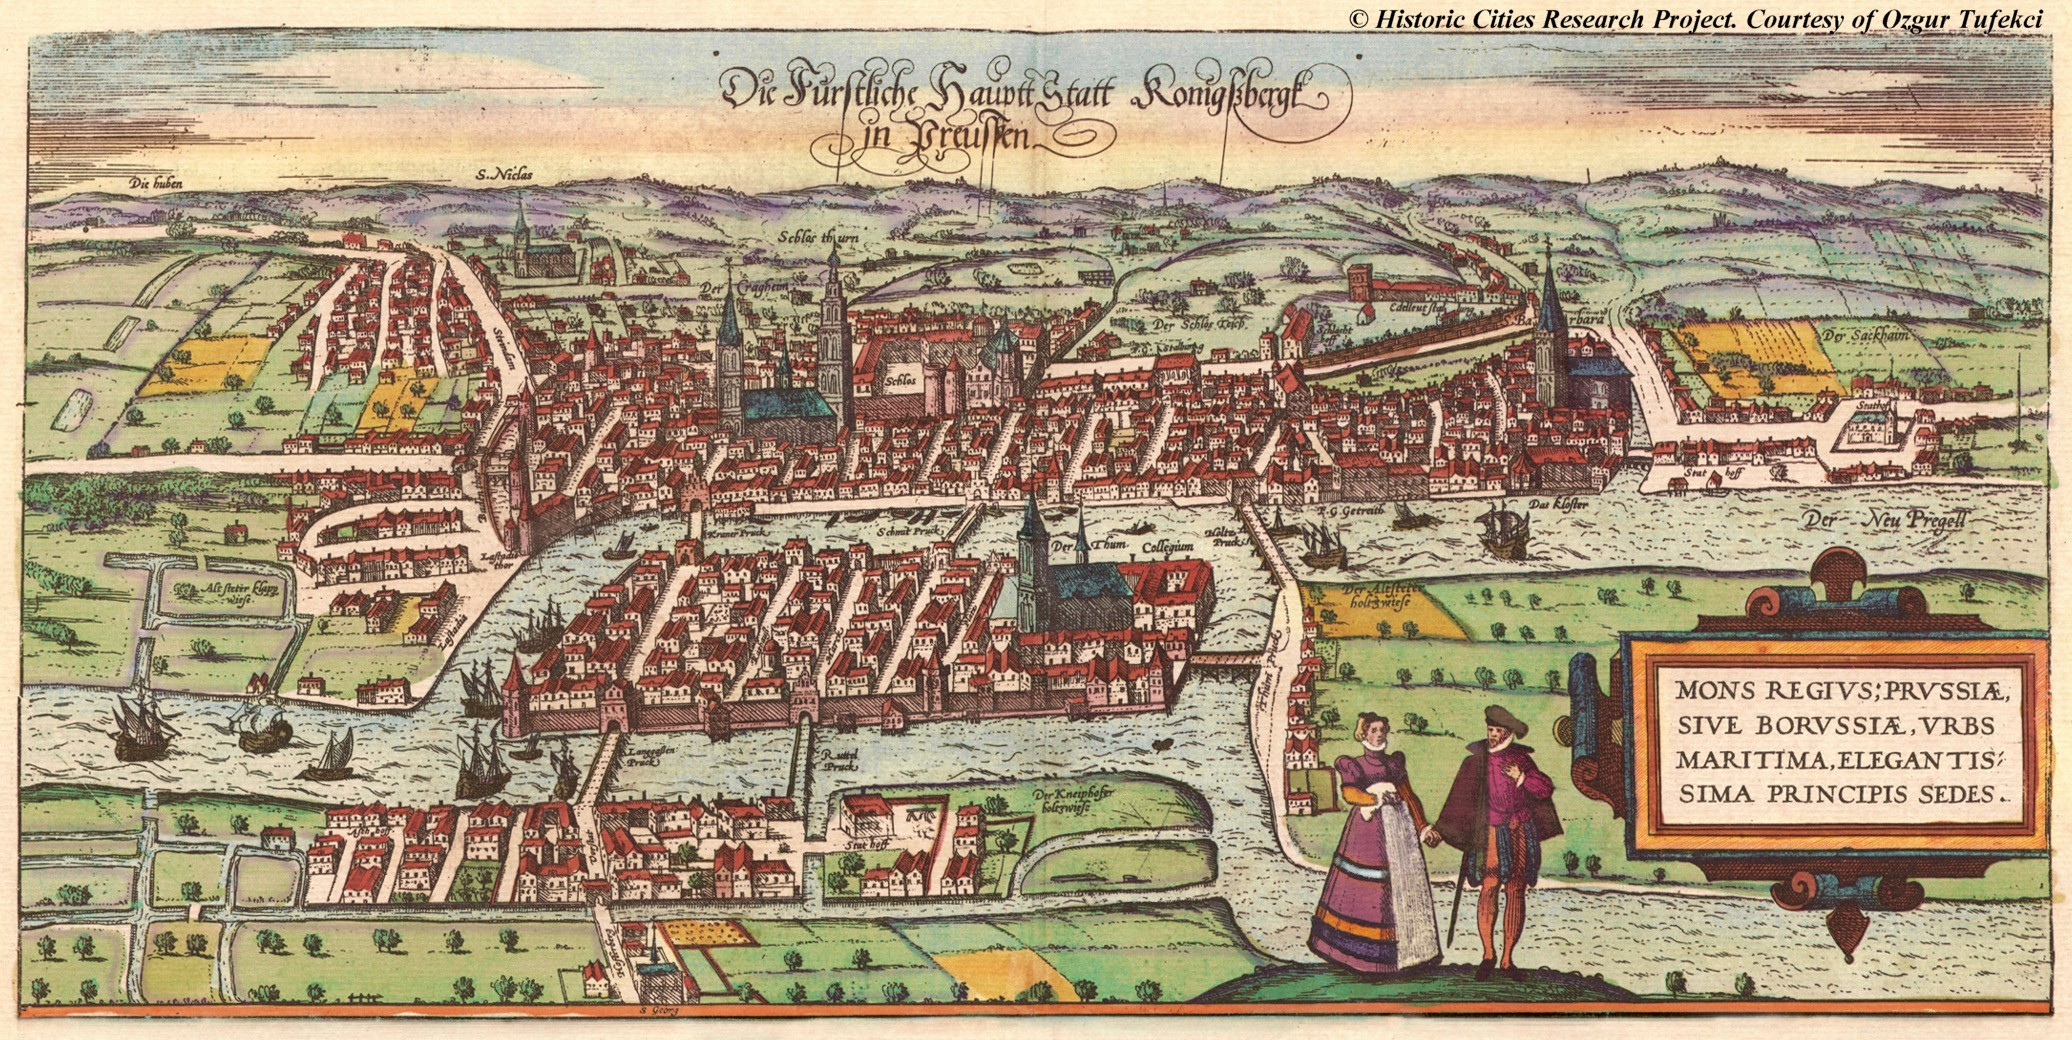
\includegraphics[width=1\textwidth]{images/konigsberg.jpg}
\end{minipage}\begin{minipage}[b]{0.48\textwidth}
\centering
\begin{tikzpicture}
    \tikzset{LabelStyle/.style= {draw}}
    \GraphInit[vstyle=Normal]
    \node[VertexStyle](A){a};
    \node[VertexStyle,right=of A](B){b};
    \node[VertexStyle,right=of B](C){c};
    \node[VertexStyle,above= 1.2cm of B](D){d};
    \draw[EdgeStyle](B) to node[LabelStyle]{} (D);
    \tikzset{EdgeStyle/.append style = {bend left}}
    \draw[EdgeStyle](A) to node[LabelStyle]{} (B);
    \draw[EdgeStyle](B) to node[LabelStyle]{} (A);
    \draw[EdgeStyle](B) to node[LabelStyle]{} (C);
    \draw[EdgeStyle](C) to node[LabelStyle]{} (B);
    \draw[EdgeStyle](A) to node[LabelStyle]{} (D);
    \draw[EdgeStyle](D) to node[LabelStyle]{} (C);
\end{tikzpicture}
\end{minipage}
\caption*{\textsf{The city of K{\"o}nigsberg in an old postcard with its graph-theoretical representation, where the bridges are the edges of the graph and the city parts are represented by nodes. This city inspired Euler to start graph theory.}}
\end{figure}

%%%%%%%%% INTRO GENERALE COMPLEX NETWORKS
\section{Complex networks science and the brain}\label{sec:complexnetworksciencebrain}
The brain is an extremely complex organ, whose dynamics is driven by the internal activity of its constituents, the neurons, responding adaptively to an ever-changing outside environment.
The neurons interact over the organic substrate that they themselves define, and shape an extremely intricate pattern of electrical and metabolic activities, giving rise to the outstanding set of abilities and possibilities typical of most evolved organisms.
Nonetheless, the notion that brain function can be reduced to the single operations of its constituents is as flawed as its complementary idea that cognition can be understood without making reference to its biological substrate.
Instead, what science is increasingly recognizing is that, for the description of most systems in nature, it is necessary to remain within a certain level of complexity and to contemplate the multiple interactions of simple subsystems taken as a whole.
It is known, indeed that many systems, despite radically different at their microscopic level, share many remarkable organizational properties, when analyzed in their entirety.

A window over the formidable and irreducible complexity of the brain can thus be opened by specific theoretical tools able to account for the brain multi-scale organization, its hierarchical structure and its modular composition.
The study of brain connectivity has already made possible many advances in neuroscience, from the identification and structural characterization of the cytoarchitecture, to the macro-scale connectivity at level of nerve fibers.
Specifically, the analysis of the architecture of the nervous system is based on the idea that the brain can be thought as a complex system at different spatial and time scales. In this respect, the tools of network theory are the method of election in the analysis of complex systems.

%%%%%%
\bigbreak

The methods of network theory date back to the problem of K{\"o}nigsberg bridges, in 1735, when the famous mathematician Leonhard Euler was faced with the problem of finding a path through the city that would cross all the seven bridges just once.
Since then a large amount of knowledge has been accumulated on networks, in what is nowadays known as graph-theory.

In totally general settings, simple graphs are usually defined as a set of nodes, entities representative of some object, connected by a set of links, denoting the strength of the relation between pairs of nodes.
Graphs can be used to represent any type of relation between interacting elements and the idea that graph-theory can be applied to brain networks has been pioneered starting from the middle nineties of the twentieth century, defining a new specialization of systems biology, dubbed \emph{network neuroscience}.

The network neuroscience relies upon the treatment of the brain as a graph, whose nodes are indicative of particular brain regions connected by links displaying the strength of their mutual interactions. The classical pipeline for the definition of a brain graph is given in Figure~\ref{fig:bullmore2009pipeline}.
In this framework, the modeling of brain in terms of graphs starts from the definition of its nodes. These can be defined as electroencephalography or multi-array electrodes or as anatomically defined regions of histological, MRI or diffusion tensor imaging data.
A clear delineation of network nodes, is one of the first steps in the whole pipeline of the graph-theoretical analyses and is highly important for the subsequent statistics resulting from the data.
The second step in the definition of a brain network is an estimate of the continuous association between nodes. The links of the graph indeed measure the interregional coordination or similarity between nodes.
To be more specific in the case of fMRI studies of resting state functional connectivity, link weights are defined as interregional temporal correlations in the fluctuations of the BOLD signals\footnote{Blood Oxygen Level Dependent, a neuroimaging technique that relies on changes in the level of oxygen in the human brain induced by alterations in blood flow.}, and the resulting graph can be represented by an adjacency matrix where the strongest correlations indicate the presence of a link between any two specific areas.
In other applications like Diffusion Tensor Imaging, a technique that is able to show the effective directions of nervous fibers traits in the brain, one can see the links as directly proportional to the number of white matter tracts connecting any two regions.
In addition, brain networks have also been defined on the basis of inter-subject anatomical covariance~\cite{evans2013,he2007}, co-activation of different brain regions across individuals subjected to experimental tasks~\cite{crossley2013a}, pharmacological challenges~\cite{schwarz2007,schwarz2008} or spectral coherence of EEG electrical time-courses.
All of these networks are ``weighted'' by definition, i.e. their links are associated with real numbers representing a measure of the strength of pairwise interactions between nodes.

%% FIGURA BULLMORE
\begin{figure}[htb!]
\centering
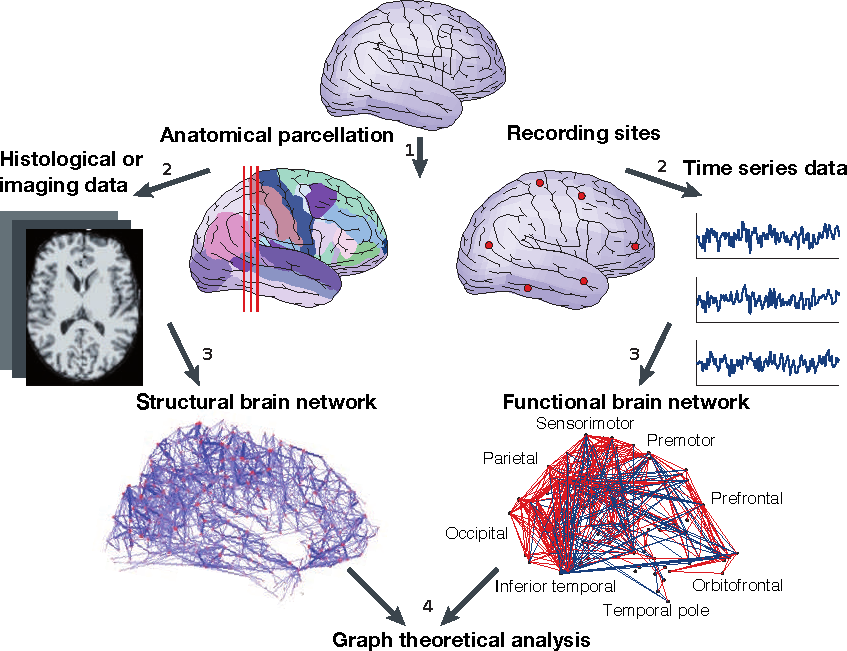
\includegraphics[width=1.0\textwidth]{images/bullmore_2009_pipeline.pdf}
\caption{Structural and functional brain networks can be explored using graph theory through four steps.}
\label{fig:bullmore2009pipeline}
\end{figure}

The ascendancy of the network neuroscience in the last decade, is driven by the evidence that almost independently from how the networks links are defined, brain networks share some common tracts at many spatial and temporal scales.

Among these findings we can mention for example, that they exhibit the \emph{small-world} property~\cite{watts1998,sporns2002,sporns2004a}, in other words, most nodes in a graph can be reached from any other node in just a few hops. To mention the importance of such topological network traits, for example small-worldness in brain networks~\cite{vandenheuvel2008} has been found to positively correlate with higher IQ in humans~\cite{vandenheuvel2009}, suggesting that human intellectual performance is likely to be related to how efficiently our brain integrates information between multiple brain regions.

Other measures have been correlated with phenotypic and structural traits.
\emph{Rich-clubs} are subset of high degree nodes who are very \emph{rich} in connections and form a communication backbone that, is hypothesized, might be valuable in supporting high-level and more cognitively advanced forms of information processing~\cite{collin2014}. Moreover, it's thought that the presence of a rich club increases the diversity of the functional repertoire over and above the effects produced by scale free type topology alone~\cite{senden2014}.
Forms of rich-club organization has been observed in cats, macaque and humans~\cite{vandenheuvel2011,harriger2012,dereus2013a,collin2014}, comprising portions of prefrontal, parietal, temporal and insular cortex. Rich club nodes and edges participate in a large number of short paths across the network, contributing disproportionately to global communication. 
Abnormal rich-club connectivity is hypothesized to be related  to familial vulnerability for schizophrenia~\cite{collin2014impaired}.
From the functional point of view, central hubs of rich clubs are concentrated in heteromodal association cortices, areas that receive input from multiple unimodal sensory association areas and/or other heteromodal cortices~\cite{kandel2013}. Contrarily, primary sensory cortices have low topological centrality and degree, therefore damage to primary sensory areas only affect them locally, while perturbation to the rich-club backbone has diffuse and severe effects on the whole network architecture~\cite{honey2008}.

More generally, network neuroscience has matured the ability not only to map alterations at the level of structural or functional connectome, but recently it started predicting and generating hypotheses about underlying pathophysiological mechanisms of disease. Clinically useful predictions are now being made on the basis of network indicators, viewed as biomarkers of brain alterations~\cite{fornito2015}.

Am important factor when considering the effects of external perturbations on brain functioning is the degeneracy (or redundancy) of network nodes. Indeed, area that are buried inside a dense module have high degeneracy, as removal of a vertex is unlikely to affect the communications between the others. A poorer prognosis is registered instead when the interested area of the insult has low degeneracy, i.e. only that area is deputed to a particular region such that no other area may compensate.
Additionally, a severe impairment of neurocognitive functions is associated with damage to highly central nodes, as depicted qualitatively in Figure~\ref{fig:prognosis_centrality}.

\begin{figure}[htb!]
\centering
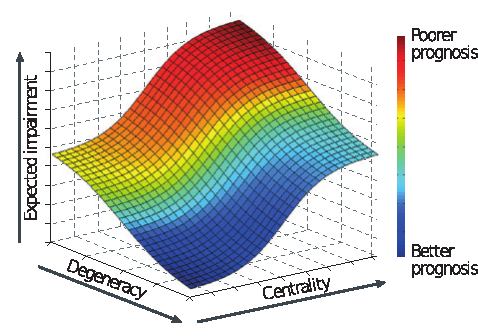
\includegraphics[width=0.75\textwidth]{images/prognosis.pdf}
\caption{Hypothetical relation between centrality of node subjected to an pathological insult, its degeneracy and the expected functional impairment.}
\label{fig:prognosis_centrality}
\end{figure}

Across the many other properties that graphs exhibit and that are arguments of further analysis \emph{per se}, one of the most directly observable is that, nodes group together forming some kind of \emph{clusters}.
At this level of meso-scale organization, the topological properties of nodes are more dependent on their neighborhood than on the rest of the graph. When the mesoscopic structure tends to group nodes with similar properties, the meso-scale structure is called \emph{assortative}. Such graphs with assortative structures consist in tightly connected groups of nodes that are themselves loosely connected with other groups. These groups are therefore dubbed as \emph{communities}. 

The organization into communities is one of the most studied properties of networks and a large amount of literature has grown on community detection, as proven by the large review of Fortunato~\cite{fortunato2010}.
The problem of detecting the communities, or ``graph-partitioning'' in the computer-science jargon, is of big theoretical and practical importance.
From the theoretic point of view, communities in networks are representative of the generative probabilistic model underlying the formation of links~\cite{karrer2011} and tell much about the statistical properties of the networks.
On the other side, practical applications of community detection are fundamental in sociology, computer science, biology and many other fields.

It's being increasingly understood indeed, that like many other information processing systems, the brain exhibit a modular architecture.
Within the modules the information is processed locally and is then shared between modules on a communication backbone~\cite{dereus2013a,vandenheuvel2013a}.

Additionally, the modular organization is exhibited hierarchically at different scales, with modules inside modules, a construction that is thought to confer robustness and adaptability to the network~\cite{meunier2010}. This kind of structure implies that modules of heterogeneous size are present at the same time in the brain networks and that an efficient method to detect the presence of large and small modules at the same time together is in order.

Several methods have been proposed to resolve the community structure of complex networks~\cite{fortunato2010,lancichinetti2009,fortunato2016}.
Many of these methods involve the definition of a fitness function that assigns positive or negative scores to edges connecting nodes within or outside the same community, and heuristics to find the optimal partition of the network that maximize this fitness function.
Among all the methods, the most popular approach is Newman's ``Modularity maximization'' and variations thereof~\cite{newman2006}.

Following the first demonstration by~\cite{schwarz2008}, partitioning of brain networks using Newman's Modularity has been widely applied to assess the brain modular structure.
A few, large modules, including the Default Mode Network, the central network, occipital and fronto-parietal networks have been observed with remarkable consistency across subjects and studies~\cite{meunier2010,wang2010}. 

Despite its popularity and merits, Newman's approach presents some important limitations.
Already at an early stage, Modularity-based methods were shown to suffer from a resolution limit, as they fail to identify modules that are smaller than a scale that depends on the size of the overall network~\cite{fortunato2007}.
As a consequence, even unambiguously defined modules, like almost complete sub-graphs or even cliques\footnote{Graphs where all nodes to connect to all nodes}, may be unduly merged into larger communities when they are too small compared to the size of the network.
Subsequent work by various groups has shown that the resolution limit is quite pervasive~\cite{lancichinetti2009,traag2011,squartini2015,lancichinetti2011,kawamoto2015}, and affects, to a different extent, many other methods, including Reichardt and Bornholdt’s~\cite{reichardt2006}, Arenas and Gomez'~\cite{arenas2008}, Ronhovde and Nussinov's~\cite{ronhovde2009}, Rosvall and Bergstrom's (\emph{Infomap})~\cite{rosvall2008,kawamoto2015} and others.

Fixes have been proposed to circumvent the resolution limit, including the introduction of a tunable parameter that enables analysis of the network at an adjustable resolution level~\cite{reichardt2006,ronhovde2010,yeo2011} or smart adjustment and rescaling of edge weights~\cite{berry2011}.
However, this requires prior knowledge of the expected size of the communities for the tuning of the resolution parameter. Moreover, it has been shown that an  adjustable resolution parameter may reduce the tendency to merge small clusters, but only at the cost of unduly splitting large clusters~\cite{lancichinetti2011}. Adjustment of the resolution parameter is an attempt to balance these two biases, but multi-resolution methods fail to recover community structures comprising heterogeneous distributions of cluster sizes~\cite{lancichinetti2011}. 
However, real-world networks (especially brain networks) are characterized by the coexistence of clusters of very different sizes, and no single parameter can adapt to the variety of network topologies observed in nature.
Hence, the resolution limit represents a critical shortcoming for the study of brain networks and is likely to have affected many of the studies reported in the literature.

\bigbreak
A short and self-contained tutorial to the jargon of graph theory is in order before delving into the details of community detection and the illustration of how the resolution limit negatively affected many neuroscientific studies.

In this introductory chapter, section~\ref{sec:elementsofgraphtheory}is devoted to the introduction to the mathematical concepts of graph theory. Section~\ref{sec:communitydetectioninnetworks}, presents the main approaches currently in use for community detection in networks. The Newman's Modularity and the null model upon which it's based is discussed in~\ref{sec:newman_modularity}.
The unavoidable consequences of Modularity maximization i.e the resolution limit and degeneracy are discussed thoroughly in section~\ref{sec:resolutionlimit} and ~\ref{sec:degeneracy}.


%%%%%%%%%%%%%%%%%%%%%%%%%%%%%%%%%%%%%%%%%%%%%%%%%%%%%%%%%%%%%%%%%%%%%
%%%%%%%%%%%%%%%%%%%%%%% ELEMENTS OF GRAPH THEORY %%%%%%%%%%%%%%%%%%%%%%%%%%%
%%%%%%%%%%%%%%%%%%%%%%%%%%%%%%%%%%%%%%%%%%%%%%%%%%%%%%%%%%%%%%%%%%%%%
\section{Elements of graph theory}\label{sec:elementsofgraphtheory}
Here we provide to the reader the basic mathematical tools to understand graph theory. We adopt the typical notation used in other works of the network science field~\cite{newman2010book,estrada2011}.


\noindent\textbullet \,A \emph{graph} $G=(V,E)$ is a representation of a set $V$ of $n$ nodes, also called \emph{vertices}, connected by $m$ links, also called \emph{edges}, in a set $E$ (Figure~\ref{fig:simple_unweighted_graph}).

\noindent\textbullet \,A graph with no multiple links and no self-loops is dubbed \emph{simple graph}.
If multiple links exist between two nodes, the graph is called \emph{multigraph}.
Additionally if a node links itself, the graph is called \emph{loopy graph}.
Figure~\ref{fig:loopy_multigraph} shows the combination of a multigraph and a loopy graph: a loopy multigraph.
If the direction of the links is important, the graph is called \emph{directed}, as shown in Figure~\ref{fig:directedgraph}, otherwise the graph is called \emph{undirected}.

\begin{figure}[htb!]
\centering
	\begin{subfigure}[hb]{0.4\textwidth}\centering
		\includegraphics[width=0.75\textwidth]{standalonetikz/tikz_simple_graph.tikz}
		\caption{}
		\label{fig:simple_unweighted_graph}
	\end{subfigure}
	\begin{subfigure}[hb]{0.4\textwidth}\centering
	\includegraphics[width=0.75\textwidth]{standalonetikz/tikz_weighted_graph.tikz}
	\caption{}
	\label{fig:simple_weighted_graph}
	\end{subfigure}
	\begin{subfigure}[hb]{0.4\textwidth}\centering
	\includegraphics[width=0.75\textwidth]{standalonetikz/tikz_loopy_multigraph.tikz}
	\caption{}
	\label{fig:loopy_multigraph}
	\end{subfigure}
	\begin{subfigure}[hb]{0.4\textwidth}\centering
	\includegraphics[width=0.75\textwidth]{standalonetikz/tikz_directed_graph.tikz}
	\caption{}
	\label{fig:directedgraph}
	\end{subfigure}
	\caption{Classes of graphs. {\textbf (a)} is a simple unweighted undirected graph. {\textbf (b)} is a simple weighted undirected graph, {\textbf (c)} is an unweighted loopy multigraph, {\textbf (d)} is a simple directed graph.}
\end{figure}

\noindent\textbullet \,The adjacency matrix $\mathbf{A}=\{A_{ij}\} \in \{0,1\}^{n \times n}$ of a binary (undirected) graph is a square $n\times n$ symmetric matrix with elements $A_{ij}=1$ when an edge exists between vertex $i$ and $j$ and $0$ otherwise.

\noindent\textbullet \,An \emph{edge-weighted graph} (also called weighted graph) $G=(V,E,\omega)$ is a graph that has a set of weights $\omega$ on the links (Figure~\ref{fig:simple_weighted_graph}). Although not true in general, we consider only weighted undirected graphs with symmetrical real adjacency matrix, meaning that if an edge exists between node $i$ and $j$ the weight from $i$ to $j$ is the same as the weight from $j$ to $i$: $\omega_{ij}=\omega_{ji}$. The weighted adjacency matrix,  indicated as $\mathbf{W}=\{ \omega_{ij} \} \in \mathbb{R}^{n\times n}$ is a real, square $n \times n$ symmetric matrix.

\noindent\textbullet \,The simplest property of the graph, once defined nodes and edges, is the \emph{density} $\rho$. It is defined on a simple graph as the ratio of the number of edges over all possible edges:
\begin{equation}
\rho = \frac{m}{\binom{n}{2}} = \frac{2m}{n(n-1)}.
\end{equation}
\noindent\textbullet \,A \emph{dense} graph is a graph where almost every possible pair of nodes is connected with an edge. Conversely, a graph is termed \emph{sparse} if the density is low, meaning that also the adjacency matrix is sparse and the number of edges has the order of magnitude of the number nodes $m ~\approx \mathcal{O}(n)$.

\noindent\textbullet \,The number of edges incident to a node in a simple graph is called \emph{degree}, denoted as $k_i$. Every half edge incident to a node is called \emph{stub}. To a vertex with degree $k_i$ then are associated $k_i$ stubs.

\noindent\textbullet \,On simple weighted graphs, the sum of weights of the edges incident to a vertex $i$ is called \emph{strength} and is denoted as $s_i$. 
In matrix terms, degree and strength are the sums over rows of the adjacency matrix $d_i=s_i=\sum_{j=1}^n A_{ij}$. It must be noted that degree and strength are equal on binary graphs, but different for weighted graphs.

\noindent\textbullet \,The \emph{degree sequence} $\{k_i\}$ $\forall i=1,\ldots,n$ is the sequence  of the degrees of the nodes, with these numbers put in ascending order, and repetitions if needed. By the \emph{handshaking lemma}~\cite{leiserson2001}, the sum of all node degrees is equal to twice the number of links:
\begin{equation}
\label{eq:handshaking_lemma}
\sum_{i=1}^n k_i=2 |E|,
\end{equation}
consequently the \emph{average node degree} is given by
\begin{equation}
\left< k \right> = \frac{2m}{n}.
\end{equation}

\noindent\textbullet \,The \emph{neighborhood} of node $i$ is the set $\Gamma_i=\{j \in V | (i,j) \in E \}$. In other words, the neighbor nodes of $i$ are the nodes which share and endpoint edge to $i$. 

\noindent\textbullet \,A \emph{path} in a graph is a sequence of edges such that the destination of each edge in the sequence is always the source of the following edge. A \emph{cycle} is a closed path, i.e. a path where the origin and destination nodes are the same.

\noindent\textbullet \,A graph that has all the possible links, indicated by $K=(V,V\times V)$ is called \emph{complete graph} or \emph{clique} (Figure~\ref{fig:completegraph}). Complete graphs on $n$ nodes, indicated as $K_n$ have a total of $m=\binom{n}{2}$ edges and density equal to $1$.

\noindent\textbullet \,The complementary graph $\bar{G}$ is the graph that has edges where $G$ has no edges and vice-versa, formally $\bar{G}=(V,V\times V - E)$.
The \emph{empty graph} is therefore defined as the complementary graph of the clique $\bar{K}$, as it has $n$ nodes and no edges (Figure~\ref{fig:emptygraph}). The \emph{cycle graph} $C_n$ is a graph containing a single cycle through all nodes and is the smallest connected cyclic graph (Figure~\ref{fig:cyclegraph}). A \emph{tree graph} is a graph with no cycles and exactly $n-1$ edges.

\noindent\begin{figure}[htb]
\centering
	\begin{subfigure}[t]{0.3\textwidth}\centering
		\begin{tikzpicture}
			\tikzset{LabelStyle/.style= {draw,font = \small}}
			\GraphInit[vstyle=Normal]
			\SetGraphUnit{1.5}
			\begin{scope}[rotate=18]
			\Vertices{circle}{a,b,c,d,e}
			\end{scope}
			\Edges(a,b,a,c,a,d,a,e,b,c,b,d,b,e,c,d,c,e,d,e)
		\end{tikzpicture}
	\caption{{\footnotesize Complete graph $K_5$}}\label{fig:completegraph}
	\end{subfigure}
	\begin{subfigure}[t]{0.3\textwidth}\centering
		\begin{tikzpicture}
		\tikzset{LabelStyle/.style= {draw,font = \small}}
		\GraphInit[vstyle=Normal]
		\SetGraphUnit{1.5}
		\begin{scope}[rotate=18]
		\Vertices{circle}{a,b,c,d,e}
		\end{scope}
		\end{tikzpicture}
	\caption{{\footnotesize Empty graph $\bar{K}_5$}}\label{fig:emptygraph}
	\end{subfigure}
	\begin{subfigure}[t]{0.3\textwidth}\centering
		\begin{tikzpicture}
		\tikzset{LabelStyle/.style= {draw, font = \small}}
		\GraphInit[vstyle=Normal]
		\SetGraphUnit{1.5}
		\begin{scope}[rotate=18]
		\Vertices{circle}{a,b,c,d,e}
		\end{scope}
		\Edges(a,b,b,c,c,d,d,e,e,a)
	\end{tikzpicture}
	\caption{{\footnotesize Cycle graph $C_5$}}\label{fig:cyclegraph}
	\end{subfigure}
\end{figure}

\noindent\textbullet \,A subgraph $\mathcal{G}$ of a graph $G$ is said to be \emph{induced} if, for any pair of vertices $i$ and $j$ of $\mathcal{G}$, the pair $(i,j)$ is an edge of $\mathcal{G}$ if and only if $(i,j)$ is also an edge of $G$. In other words, $\mathcal{G}$ is an induced subgraph of $G$ if it has the most edges that appear in $G$ over the same vertex set. If $\mathcal{G}$ is chosen based on a vertex subset $S$ of $V(G)$, then $\mathcal{G}$ can be written as $G[S]$ and is said to be induced by $S$.

\noindent\textbullet \,A simple graph is said \emph{connected} if there exist a path between any pair of nodes. If the graph itself is not connected, then it is formed by a set of connected subgraphs, also called \emph{weakly connected components}.


%%%%%%%%%%%%%%%%%%%%%%%%%%%%%%%%%%%%%%%%
\subsection{Clustering}\label{sec:clustering}
Grouping nodes according to some criterion of similarity between them is the basis of the formation of clusters in networks.
\noindent\textbullet \,A set of mutually disjoint, induced subgraphs that covers all the nodes is called a \emph{clustering}.
A clustering $\zeta = \{\zeta_c\}$ of $G$ is a partitioning of the set $V$ into $C$ disjoint sets of nodes, $\zeta_c \subseteq V$, which we call \emph{modules} or \emph{communities}, interchangeably. 
Each module is a node-induced subgraph $\mathcal{G}:=(V[\zeta_c],E[\zeta_c])$, also indicated as $G[\zeta_c]$.

\noindent\textbullet \,We denote the number of nodes of the module $G[\zeta_c]$ with $n_c$, the number of edges with $m_c$ and the total number of pairs of nodes with $p_c=\binom{n_c}{2}$.
From the notational point of view, a clustering can alternatively be defined with a \emph{node assignment vector} $\sigma \in \mathbb{N}^n$ in which every node is assigned to an integer label representing the community index. 

\noindent\textbullet \,The \emph{Kronecker delta} on the assignment vector $\delta(\sigma_i,\sigma_j)=1$ indicates when two nodes lie in the same module and $\delta(\sigma_i,\sigma_j)=0$ when they belongs to different modules.

\noindent\textbullet \,The \emph{internal degree} $k_{\textrm{int}}(i)$ of vertex $i$ in the module $\mathcal{G}$ is the number of edges connecting $i$ to other vertices in $\mathcal{G}$. If $k_{\textrm{ext}}(i)=0$, the vertex has neighbors only within $\mathcal{G}$, on the other hand if $k_{\textrm{int}}(i)=0$, the vertex is disjoint from $\mathcal{G}$ and should not be part of the same community.

\noindent\textbullet \,The \emph{external} degree $k_{\textrm{ext}}(i)$ of vertex $i$ in the module $\mathcal{G}$ is the number of edges connecting $i$ to vertices not in $\mathcal{G}$.

\noindent\textbullet \,The \emph{subgraph internal degree} $K_{\textrm{int}}(\mathcal{G})$ is the sum of the internal degrees of its vertices.
Likewise, the \emph{subgraph external degree} $K_{\textrm{ext}}(\mathcal{G})$ is the sum of the external degrees of its vertices.

\noindent\textbullet \,The \emph{subgraph total degree} $k(\mathcal{G})$ is the sum of the degrees of the vertices of $\mathcal{G}$. By definition, $K(\mathcal{G}) = K_{\textrm{ext}}(\mathcal{G}) + K_{\textrm{int}}(\mathcal{G})$. For convenience of notation we will denote without loss of generality $K_{\textrm{int}}(\mathcal{G}[ \zeta_c ])$ as $K_c$, specifying the full notation where is needed.

\begin{figure}[htb]\centering
\begin{tikzpicture}
	\GraphInit[vstyle=Normal]
	\SetGraphUnit{1.5}
	\Vertices{circle}{a,b,c,d,e}
	\Edge[label=1](a)(b)
	\Edge[label=2](a)(c)
	\Edge[label=0.5,style={pos=0.25}](a)(d)
	\Edge[label=3](a)(e)
	\Edge[label=1](c)(b)
	\node[draw=black!50,dashed,rounded corners=5mm,fit=(b.north) (a.south) (c.west) (a.east)](BORD) {};
	\node[left of=BORD,anchor=east, inner sep=1cm]{$\mathcal{G}$};
\end{tikzpicture}
\caption{Internal degree $k_{\textrm{int}}(a)=2$, internal strength $s_{\textrm{\textrm{int}}}(a)=3$, external degree $k_{\textrm{ext}}(a)=2$, external strength $s_{\textrm{ext}}(a)=3.5$.}
\label{fig:internaldegree}
\end{figure}

\noindent\textbullet \,The \emph{intracluster density} of the subgraph $\mathcal{G}$ is defined as the ratio of the intracommunity edges over the number of pairs 
\begin{equation}
\rho_{\textrm{int}}(G)=\frac{m_c}{p_c} = \frac{2 m_c}{n_c(n_c-1)}.
\end{equation}

\noindent\textbullet \,The \emph{inter-cluster density} is instead defined as the ratio of edges with one endpoint in $\mathcal{G}$ and the other in $G-\mathcal{G}$, over the total possible number of edges connecting $\mathcal{G}$ with the rest of the graph: 

\begin{equation}
\rho_{\textrm{ext}}=\frac{m-m_c}{n_c(n-n_c)}.
\end{equation}

\noindent\textbullet \, The total intracluster edges and total intracluster node pairs numbers are the sum over all modules $c$ of intracommunity edges and node pairs:
\begin{align}
&m_\zeta= \sum \limits_{c=1}^C |E[\mathcal{G_c}]| = \sum \limits_{c=1}^C m_c \\
&p_\zeta= \sum \limits_{c=1}^C \binom{|V[\mathcal{G_c}]|}{2} = \sum \limits_{c=1}^C p_c.
\end{align}

\subsection{Communities}\label{sec:communities}
The word \emph{community} applied to complex networks originated in sociology as groups of people tend naturally to form groups: family, friends, acquaintances. Social communities then can be thought as subgroups of people knowing each other more probably than with other external people. 
The problem of community definitions, although intuitive at first sight, is multifaceted and ambiguous as no universally accepted definition of network community exist as some degree of arbitrariness and common sense is required, a feature that is difficult to describe quantitatively. 
Importantly, the identification of communities is possible for sparse graphs. On dense graphs, the community detection problem requires different tools, close to those of data clustering, with different concepts and definitions.

Among all the notions of communities two different families can be identified. The \emph{local definition} involve that a community is viewed as a separate entry, an autonomous module: the community is studied as isolated from the graph as a whole.
Such definition imply that the corresponding communities are mostly maximal subgraphs, subsets of nodes that cannot be enlarged with the addition of new nodes or edges without altering the very same property upon which they are defined.
The most important local criterion for communities definition are the \emph{complete-mutuality}, the \emph{reachability}, the comparison of vertex degree and \emph{internal-external cohesion}~\cite{wasserman1994,alba1973}. Complete mutuality means that the identified community is a clique as every node is mutually connected with all the others. Reachability implies that there exist a path between every pair of nodes in the community. Finally, the internal- external cohesion concept is equivalently represented by the Radicchi's definitions of \emph{strong communities}~\cite{radicchi2004}.

For a community $\mathcal{G}$ to be defined in \emph{strong} sense, every node in the community must exhibit a larger internal degree than external degree. The concept is made quantitative in the following definition (Eq.~\ref{eq:strongcommunities}):
\begin{equation}\label{eq:strongcommunities}
\forall i \in V[\mathcal{G}] \qquad k_{\textrm{int}}(i) > k_{\textrm{ext}}(i).
\end{equation}
The strong community criterion is extremely stringent and most real-world networks do not exhibit such property, even the simplest.
It is possible though to weaken this constraint, asking that \emph{on average} the internal degree is greater than the external degree.  Upon this idea the concept of \emph{weak communities} is built (Eq.~\ref{eq:communityweak}):
\begin{equation}\label{eq:communityweak}
\sum \limits_{i \in V[\mathcal{G}]} k_{\textrm{int}}(i) > \sum \limits_{i \in V[\mathcal{G}]} k_{\textrm{ext}}(i)
\end{equation}
Finding strong communities is more difficult than finding weak communities and most algorithms fail in this job, as most of them have their own concept of community. Nonetheless these two last definitions are almost universally accepted and give a precise idea of the meaning of community. Additionally, the weak criterion of community is the basis of the planted-partition model~\cite{condon2000} and its later modifications~\cite{lancichinetti2008} that we'll encounter in the next sections. 

The \emph{global definition} are based on an interpretation of the network as a whole, whose communities are an essential part of it, which cannot be taken apart without destroying its connectivity. Most of the global criteria of communities encompass global property of the graph that are used by algorithm to deliver a modular decomposition, in this sense the global definitions are always indirect, often based on \emph{null models} or for example on dynamical processes on the network (random walkers~\cite{pons2006} or more complex processes such those described by the map equation  Infomap~\cite{rosvall2008}).

Apart from global or local definitions of communities is the indication that multiple different sub-networks in brain FC networks have been observed consistently with a variety of analysis techniques~\cite{fox2005,deluca2006,schwarz2007} such as ICA or other multivariate methods.
This empirical evidence, shown not only in humans but also in higher vertebrates such as cats~\cite{scannell1995} and macaques~\cite{felleman1991}, suggests that to some extent the high level functional organization is based on the balance of two competing principles of segregation and integration.
The nervous system is obviously shaped by this balance as the need of fast information processing is satisfied by small-scale neuronal circuits, typically at the first stages of sensory input processing (e.g. the very localized functional area of visual processing V1 or the primary motor cortices), while at larger scale the cortex works in concert connecting all the segregated areas in a larger, widely distributed complex network.
It is more and more recognized~\cite{tononi1994,tononi1998,deco2015} that complex behaviors arise thanks to the dynamical interplay of the integrated and segregated actions of different regions of the brain.

The network communities and hubs support this segregation-integration balance. Recently, experiments in which computational dynamical processes are simulated over the topology of the whole-brain networks~\cite{deco2015} have shed light over the role of communities in shaping the cortical activity. Indeed it was found that the network communities consist in the areas that are devoted to the segregated information processing, while the hubs (and the rich clubs) are deputed to convey that information over the whole brain.

Among the many advantages that a modular organization of the brain benefits, two are of greatest importance. The organization of a system into many compartments devoted for different roles (and possibly with some level of overlap) is surely an evolutionary advantage. 
Keeping the system compartmentalized can limit the influence of external sources of perturbation, thus bounding the interdependence of biological processes going on in each unit. Computational and evolutionary studies have indeed shown that a modular organization emerges spontaneously, promoting flexibility to an ever-changing outside environment~\cite{kashtan2005,kashtan2007} and maximizing bidirectional information exchange between neural populations~\cite{yamaguti2015}.
An external environment that keeps changing, forces organism to quickly adapt and to develop modules apt to respond adaptively to the outside driving forces.
As the goals where changing with time during evolution, the naturally evolved subnetworks, were not ``written'' every time from scratch, but were only rewired slightly in order for other parts to be built that connected the previously optimal sub-routines, a practice that is paradoxically very common even in software engineering. 
Dynamics of module or patterns emergence and reuse have also been observed in bacterial metabolic networks~\cite{kreimer2008} and interestingly in non-biological networks. In the field of robotics, spontaneous structural modularity of neural networks controllers emerge from evolutionary optimization when successful robot behavior is encoded as fitness function~\cite{bongard2011}.

A second benefit for modular brain networks resides in the increased resilience to sudden external perturbations. Local disruptive modification may only affect one module, whereas the others are preserved from the insult. Both for externally or internally generated fluctuations, a modular architecture thus prevent functional disruption of the network leading to possible death of the organism. Taken together the modular architecture of brain networks is of key importance for the healthy brain.


\subsection{Nodal roles}
Every node in a network is characterized by its role in relation to other nodes. Given a clustering $\zeta$, some nodes act as bridges between two or more communities, having neighbors in one or other module. Other nodes instead share the majority of neighbors inside their same community.
To investigate differences in nodal roles as determined by different community detection methods, it's usual to attribute each node two parameters~\cite{guimera2005}.
The first, dubbed \emph{participation coefficient}, indicated by $P_i$ and included in the range $[0,1]$ reflects the extent to which a node is connected to nodes in other modules, and is defined in Eq~\ref{eq:participationcoeff} 
\begin{equation}\label{eq:participationcoeff}
P_i = 1 - \sum_c \left( \frac{k_{ic}}{k_i} \right)^2
\end{equation}
where $k_{ic}$ is the number of links of node $i$ to nodes in module $c$ and $k_i$ is the total degree of node $i$.
Converselely, the second parameter dubbed \emph{within-module degree}, indicated by $z_i$,  reflects the degree of connectivity of a node to node in its same community, and is defined as: 
\begin{equation}\label{eq:withinmoduledegree}
z_i = \frac{k_i - \left< k_{c_i} \right>}{\sigma_{k_{c_i}}}
\end{equation}
where $k_i$ is the node degree,  $\left< k_{c_i} \right>$ is the average degree of nodes in the same module $c$ of node $i$ and $\sigma_{k_{c_i}}$ the standard deviation of the degree of nodes in the same module $c$ of node $i$.

Hub classification is critical for the interpretation of the roles played by the highly connected nodes within the network structure.
The Guimera and Amaral~\cite{guimera2005} classification scheme, specifies for every node its participation coefficient and within module degree z-score, lying the nodes over a 2D cartesian space, divided in seven regions as shown in Figure~\ref{fig:gagraph}.
Depending on the specific cut-off values of participation coefficient and intra-modular connectivity, the nodes are defined as ultra-peripheral (region R1), peripheral (region R2), connector non-hubs (region R3), kinless non-hubs (region R4), provincial hubs (region R5), connector hubs (region R6) and kinless hubs (region R7). 

Naturally, connector hubs are of great importance for communication between modules (Figure~\ref{fig:brain_network_communities}).
Indeed, connector hubs are those with high values of participation coefficient and high values of within-module degree z-score.
In the context of brain networks, these hubs are responsible for integration of the different modules into a cohesive structure, and are thought to be particularly vulnerable in the presence of brain insult or disease, as damage to these nodes is likely to disrupt network connectedness.
In contrast, provincial hubs are more importantly involved in functional specialization and local processing, therefore damage to these areas should yield really specific clinical deficits, whereas damage to connector hubs results in complex and pervasive neurological dysfunctions.


\begin{figure}[htb!]
\centering
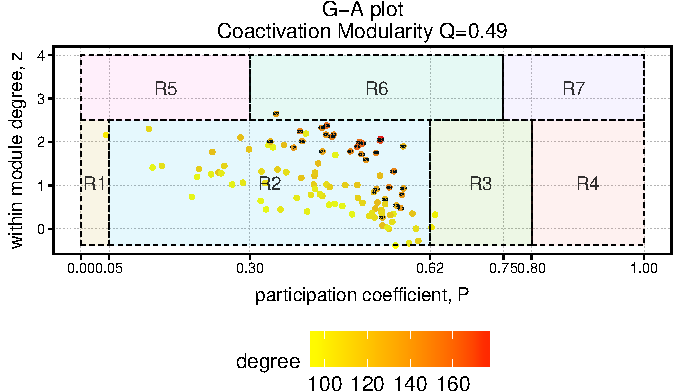
\includegraphics[width=0.75\textwidth]{images/guimera_amaral_coact_q.pdf}
\caption{Guimera and Amaral classification scheme for the modular structure induced by Modularity maximization of a co-activation network as obtained from~\cite{crossley2013a}. Each node is indicated by specific coordinates $(P_i,z_i)$ and occupies one of the seven different regions, assigning it its role. Nodes total degree is color coded with colors fro yellow to red, as shown in the legend.}
\label{fig:gagraph}
\end{figure}

\begin{figure}[htb!]
\centering
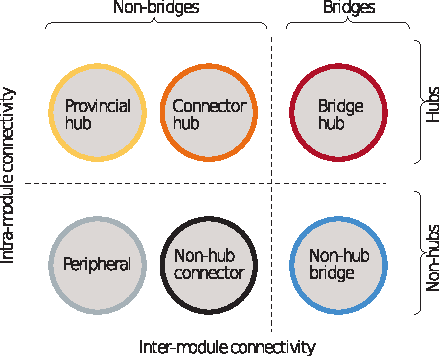
\includegraphics[width=0.5\textwidth]{images/hubs_nonhubs.pdf}
\caption{Schematic assessment of nodal roles. Interestingly under this convention, bridges represent the most extreme case of nodes, with a relatively equal distribution of connectivity between different modules. Bridges are thus best detected when overlapping communities are allowed. They bridges hubs and non-hubs occupy the R7 region of the original GA scheme. Adapted from~\cite{fornito2015}.}
\label{fig:hubs_bridges}
\end{figure}

\begin{figure}[htb!]
\centering
\hfill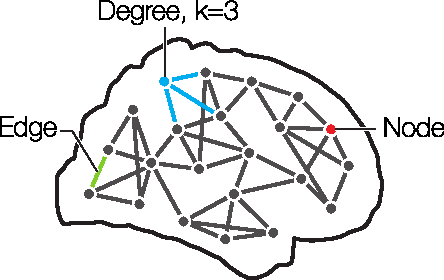
\includegraphics[height=0.25\textwidth]{images/brain_network_basics.pdf}\hfill
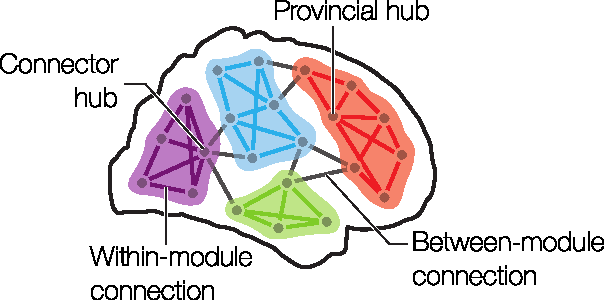
\includegraphics[height=0.25\textwidth]{images/brain_network_communities.pdf}\hfill
\caption{Meaning of communities, hubs and connectors in an artistic view. Adapted from~\cite{sporns2016}.}
\label{fig:brain_network_communities}
\end{figure}

%%%%%%%%%%%%%%%%%%%%%%%%%%%%%%%%%%%%%%%%%%%%%%%%%%%%%%%%%%%%%%%%%%%%%
%%%%%%%%%%%%%%%%%%%%%% Models of random graphs %%%%%%%%%%%%%%%%%%%%%%
%%%%%%%%%%%%%%%%%%%%%%%%%%%%%%%%%%%%%%%%%%%%%%%%%%%%%%%%%%%%%%%%%%%%%

\subsection{Models of random graphs}\label{sec:models_random_graph}
A large effort of network science is devoted to the description of the generative processes that lead to the networks observed in real-world settings. The ability to understand such generative models is of primary importance in many fields, as it enable researchers to make prediction about the behavior of the system under exam and to compare systems, gaining knowledge.
In general, a random graph is a model network in which some specific set of parameters take fixed values, but the network is random in other respects.
The theory of random graphs studies the intersection between graph theory and probability theory.
%In the first part of the twentieth century, mathematicians developed advanced theories of random graphs as they needed to compare the properties of real-world networks against random null hypotheses.
%A random graph is a probability space $(\Omega,\mathcal{F},\mathcal{P})$, where the sample space $\Omega$ is a nonempty set of graphs, the set of events $\mathcal{F}$ is a collection of subsets of the sample space (usually the power set of $\Omega$), and $\mathcal{P}$ is a function that assigns a probability to each event. It is usual to describe a random graph by a sequence of steps to construct it. Such a sequence is called an \emph{random graph model}.

%Given the unavailability of computer simulations at that time, the simplest model dates back to 1959 and is due to Erd\H{o}s and Rényi~\cite{erdos1959}. In the Erd\H{o}s-Rényi model (also called $G_{n,m}$ model, the sample space $\Omega$ is the set of all graphs having $n$ nodes and $m$ edges.
One of the simples models is the random network generated by selecting exactly $m$ edges from the possible $\binom{n}{2}$ edges and placing them at random over the nodes pairs.
This model, displaying the fixed constraint of edge number, is mathematically known as $G(n,m)$ or \emph{Gilbert} random graph.
In probabilistic terms, the $G(n,m)$ graph is equivalent to say that the network is sampled choosing uniformly from the set $\Omega$ of all $\binom{\binom{n}{2}}{m}$ possible graphs. Intuitively then it is possible to assign a probability score to each instance of a random graph model. In the $G(n,m)$, each instance is equiprobable.

Strictly speaking, a random graph model is better defined as an ensemble of networks, therefore as a probability distribution $\mathcal{P}(\Omega)$ over the space of all graphs $G$.
The Gilbert random graph model is then associated with a probability distribution sharply peaked in $\mathcal{P}(G)=1/\Omega$ for graphs with $n$ nodes and exactly $m$ edges, and zero otherwise.
Although some properties of the $G(n,m)$ models are easy to compute, like the mean number of edges (trivial), others are more complicated because of the hard constraint imposed on edges number.

A way more useful random graph model is instead due to Erd\H{o}s and Rényi~\cite{erdos1959}. 
To solve the analytical computation problems on the $G(n,m)$ model, the Erd\H{o}s-Rényi model introduces a parameter $p_{\textrm{ER}}$ that specifies the probability of an edge to exist given two nodes, rather than picking exactly $m$ edges.
Technically the $G(n,p)$ random graph model or \emph{Erd\H{o}s and Rényi} (ER) model, is the ensemble of simple graphs with $n$ nodes in which each simple graph $G$ of $m$ edges appears with probability
\begin{equation}
P(G)={p}_{ER}^{m}(1-p_{\textrm{ER}})^{\binom{n}{2}-m}
\end{equation}
Differently from the $G(n,m)$ model, because of the Bernoulli distribution of edges, this graph model is also called \emph{Bernoulli random graph} or \emph{Poissonian random graph} and generally intended as \emph{the} random graph.

As every graph obtained from the Erd\H{o}s-Rényi model is a sample from a probability space, a description in terms of ensemble averages is more appropriate.
In the ER model, the expected number of edges in such a graph is the average over $\binom{n}{2}$ independent coin tosses with probability $p_{\textrm{ER}}$:
\begin{equation}
\left< m  \right> = \binom{n}{2}p_{\textrm{ER}}
\end{equation}
and the expected degree $\left< k \right>$ is the same for every node
\begin{equation}
\left< k \right> = p_{\textrm{ER}}(n-1).
\end{equation}
The probability that a node $i$, chosen at random, has degree $k$ is called the \emph{degree distribution}. In general terms, such probability is expressed as:
\begin{equation}
\Pr(k) = \frac{\left< |\{ i \| k_i=k \}| \right>}{n}.
\end{equation}
In the ER model, a given node is connected with probability $p_{\textrm{ER}}$ to each of the other $n-1$ nodes. Thus, the probability of being connected to a particular $k$ other nodes and not to any of the others is $p^k(1-p)^{n-1-k}$, but since there are $\binom{n-1}{k}$ ways to choose those $k$ other nodes, hence the total probability of being connected to exactly $k$ others is:
\begin{equation}
\Pr(k) = \binom{n-1}{k}p_{\textrm{ER}}^k(1-p_{\textrm{ER}})^{n-1-k}
\end{equation}
a binomial distribution that can be approximated to a Poisson distribution for large $n$:
\begin{equation}
\Pr(k) \approx \frac{(n p_{\textrm{ER}})^k e^{-n p_{\textrm{ER}}} }{k!}.
\end{equation}
\bigbreak
In generalizing the concepts of random networks models, one can define every simple graph on $n$ nodes as the output of a random process where each edge $(i,j) $ is sampled with a probability $\Pr(i,j)_{ \boldsymbol \theta}$ with $\boldsymbol \theta$ a vector of hyperparameters. In the simplest case of the ER graph, this generative model is an uniform probability distribution with $\boldsymbol \theta=p_{\textrm{ER}}$ as every pair of nodes is linked by an edge with constant probability:
\begin{equation}
\Pr({i,j})_{p_{\textrm{ER}}} = p_{\textrm{ER}}.
\end{equation}

Importantly, both the ER and Gilbert models should not show any modular structure as every substructure that appears is effect of random fluctuations due to finite sampling effects. We will see, though, in the following chapters that still some algorithms find communities in ER graphs.

The ER model, although very useful as it make analytical calculation of almost all network properties really easy, does not realistically represent empirical networks.
Its Poissonian degree distribution (Figure~\ref{fig:deg_dist_poisson_er}) is far from the degree distributions seen in most of the real-world networks.
In fact, the empirical behavior of the degree distribution of real networks is one of the main reasons why they attracted so much interest from the scientific community.

The world-wide-web, as well as the connectome of the worm \emph{C. Elegans}\footnote{\emph{Caenorbiditis elegans}, a small nematode worm, famous as the first living organism whose connectome has been completely mapped.} and many other examples, shows that the degree distribution is not centered around a mean value as predicted by ER model. 

\begin{figure}
\centering
\begin{minipage}[b]{0.5\textwidth}\centering
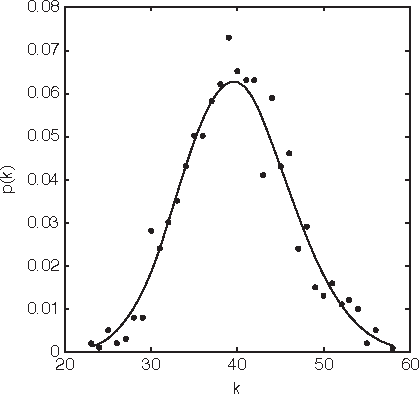
\includegraphics[height=4cm]{images/deg_dist_poisson_er.pdf}
\end{minipage}\noindent
\begin{minipage}[b]{0.5\textwidth}\centering
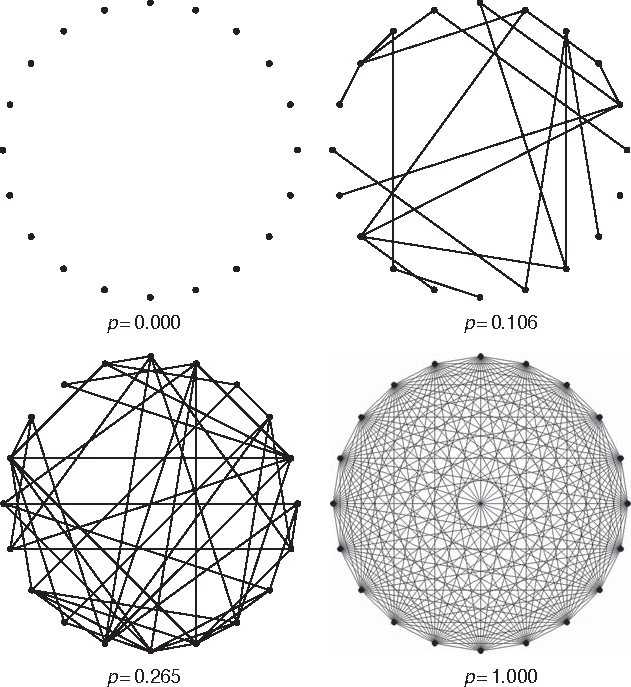
\includegraphics[height=4cm]{images/er_graphs.pdf}
\end{minipage}
\caption{Examples of ER graphs. On the left the Poisson degree distribution of an ER network, $n=1000$,$p=0.04$. On the right ER model instances at different values of $p$. Adapted from~\cite{estrada2011}.}
\label{fig:deg_dist_poisson_er}
\end{figure}

Instead, in real networks, highly connected nodes exist within a bulk of low connected nodes and the degree distribution is not decaying exponentially, thus producing the observed phenomenon of \emph{heavy tails}. Indeed, many networks display a degree distribution that follows a \emph{power-law} form
\begin{equation}
\Pr(k) \propto k^{-\gamma}
\end{equation}
where $\gamma$ is usually included in the $[2,3]$ interval.
Power-law distributions, also dubbed \emph{scale-free}, lack a specific scale. Indeed, $P(\alpha k)=f(\alpha)P(k)$ for some multiplicative constant $\alpha$  and $f$ a function of $\alpha$. Therefore, the functional form of the power-law remain unchanged.

Hence, in understanding the limitation of the Erd\H{o}s-Rényi model, researchers developed a multitude of generative models of graphs that tried to better model properties like the heavy-tails seen in power-laws or also the \emph{small-worldness} phenomenon, i.e. the observation that most nodes in a network are reachable from every other in a small number of hops.
To keep in account the features of empirical networks, other models of networks have been developed like the models of Watts-Strogatz~\cite{watts1998} model and Barabasi-Albert~\cite{barabasi1999}.

For example, in the Watts-Strogatz model a graph with groups of densely connected nodes is generated as follows:
\begin{enumerate}
\item Construct a ring with $n$ nodes and connect each node to the $l$ nearest nodes ($l/2$ in each side of the ring).
\item Choose a node $i$ and the edge $e$ that connects $i$ to its nearest neighbor in a clockwise manner.
\item With probability $p_r$ replace the edge $e$ by the edge that connects $i$ to a node taken at random according to an uniform distribution over the entire ring.
\item Repeat the steps 2 and 3 for each node in clockwise manner.
\item Choose a node $i$ and the edge $e$ that connects $i$ to its second neighbor in a clockwise sense and repeat the steps 2-4.
\item Repeat the process considering the third nearest neighbor and so on, until each edge of the original lattice has been considered.
\end{enumerate}

The resulting graph shows the property of having short average path length, although the degree distribution is not power-law.
To prevent this issue, the Barabasi-Albert graph model aims to construct graphs with a dynamic attachment process.
In the BA model, one considers a small number $n_0$ of initial nodes. Then at each step, one adds a new node and connect it to a fixed number $(\leq n_0)$ of nodes that already exist in the network. The probability that the new node will be connected to a node $i$ is then proportional to $k_i^{p_s}$,  where $p_s$ is a parameter called the \emph{scaling exponent}. That algorithm generates graphs in which the frequency of nodes with degree $k$ is asymptotically proportional to ${k}^{-3}$. This power relationship between frequencies and degrees indicates that this model accounts for the power-law distribution of degrees seen in many real networks.
Although very well studied, both models are still lacking a strong community structure and more complex models have been studied by the network science community.

\subsection{Stochastic block models}
None of the previously reported generative models explicitly accounts for the modular structure.
The modules often observed in the ER model are due to statistical fluctuations.
The BA model, too, does not take into account a block structure, when generating a power-law network and clusters in BA model are due to local structures around nodes with high degree.
To overcome these limitations, a variable encoding the block structure must be taken into account explicitly. 
The most commonly used generative model for random modular networks is called the stochastic block model (SBM)~\cite{holland1983}, which generalizes the Erd\H{o}s-Rényi random graph by giving each pair of nodes a connection probability depending only on their module affiliation $\boldsymbol \sigma$.
The SBM model tends to produce graphs containing communities, subsets characterized by being connected with one another with specific edge densities.

A stochastic block model for undirected graphs is defined by three variables: the number of nodes $n$, the set of communities in form of a membership vector $\boldsymbol \sigma$ and a symmetric square matrix  $\mathbf{B} \in \mathbb{R}^{|C| \times |C|}$ of edge probabilities between modules. In the case the matrix $\mathbf{B}$ is constant, the SBM recovers exactly the ER model.

In the case the matrix $\mathbf{B}$ takes only two different values, a model known as the \emph{planted partition model}, each pair of nodes in the same block are connected with probability $\mathbf{B}_{ij}=p_{in}$ and pairs of nodes in different modules are linked with probability $\mathbf{B}_{ij}=p_{out}$, as shown in Figure~\ref{fig:planted_peixoto}. Specific edge probability in the planted partition model is simply described as $\Pr_{ij} = p_{in}\delta(\sigma_i,\sigma_j) + p_{in}\delta(\sigma_i,\sigma_j)$.
In building the planted partition model, though one has to set in advance the number of modules $|C|$ (or blocks) and define an equal number of nodes in every module.

\begin{figure}[htb!]
\centering
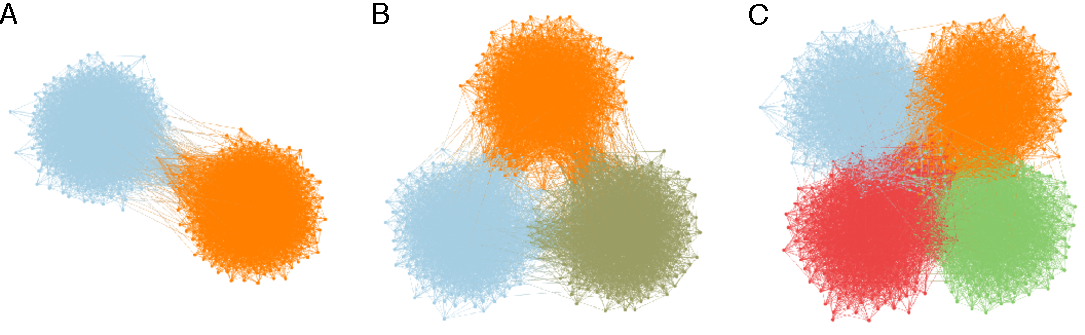
\includegraphics[width=1.0\textwidth]{images/peixoto_block_models.pdf}
\caption{Realizations of the planted partition model with different intra- and extracluster linking probabilities and number of modules. A., $|C|=2, p_{in}=0.99, p_{out}=0.025$, B. $|C|=3, p_{in}=0.98, p_{out}=0.06$, C. $|C|=4 p_{in}=0.97, p_{out}=0.12$. Adapted from~\cite{peixoto2015}.}
\label{fig:planted_peixoto}
\end{figure}

Although largely used, the planted-partition model has several drawbacks.
Indeed, as generalization of the ER model, each node has the same expected degree and all communities have the same size.
While, these properties are of great help when performing analytical calculations, they also make it badly suited for practical applications, as degree homogeneity is seldom realized in real networks.

To overcome the unrealistic settings of the planted partition model, the Lancichinetti\hyp{}Fortunato\hyp{}Radicchi (LFR) model, first described in~\cite{lancichinetti2008}, modified the planted partition model to exhibit powerlaw distribution of both node degrees and community size, with exponents $\tau_d$ and $\tau_c$ respectively, as observed in real networks.
As each realization is accompanied by the membership affiliation vector $\boldsymbol \sigma$, the LFR model has been used primarily as benchmark for evaluating the effectiveness of different community detection methods~\cite{fortunato2010,lancichinetti2009} at different level of difficulty. It was further extended to be able to generate weighted networks with overlapping modules in~\cite{lancichinetti2009a}.
The major advantage of the LFR model is the tunable level of community mixing. Indeed, each node share a fraction $1-\mu_t$ of edges with nodes in its same community and a fraction $\mu_t$ with nodes in other communities: $0 \leq \mu_t \leq 1$ is dubbed the \emph{topological mixing parameter}.
Additionally, given a degree sequence, taken by sampling the power law distribution with exponent $\tau_d$, on weighted networks a parameter $\beta$ is used to assign strength to each node: $s_i=k_i^\beta$ where the parameter $\mu_w$ is used to partition the node strength into an intra-community component proportional to $$(1-\mu_w)$$ and an inter-community component proportional to $\mu_w$: $$s_i = (1-\mu_w)s_i^{(int)} + (\mu_w)s_i^{(ext)}$$. This power-law form of node strengths is chosen to match observations on real graphs, as indicated by~\cite{barrat2004}.
The actual weights of the edges are then chosen to minimize the variance between the expected and the observed strengths by means of an iterative optimization step. Hence is possible to obtain a theoretical estimate of the average edge weights that reads:
\begin{align}
\left< w^{int} \right> = \frac{(1-\mu_w)\left< s\right>}{\frac{(1-\mu_t)\left< k\right>} = \frac{(1-\mu_w)}{(1-\mu_t)}\left < k \right>^{\beta-1} \\
\left< w^{ext} \right> = \frac{(\mu_w)\left< s\right>}{\frac{(\mu_t)\left< k\right>} = \frac{(\mu_w)}{(\mu_t)}\left < k \right>^{\beta-1}.
\end{align}
As for the planted partition model, where communities where defined as long as $p_{in}>p_{out}$, for the case of the LFR model, one asks that in order for communities to be such it must be that
\begin{equation}
\left< w^{int} \right> \geq \left< w^{ext} \right>
\end{equation}
resulting in the equivalent formulation $\mu_w  \geq \mu_t$. If this last condition is not met indeed each node would bring more weight about its connectivity on the edge weights rather than on its degree, that is why: most community detection algorithms working with weighted networks, thus would be informed of the large edge weights and are mislead considering the node as an hub even in the presence of just a few neighbors.

The modularity of the network is controlled primarily by the topological mixing coefficient. In the case $\mu_t$ is exactly zero, the network consists of isolated components and the stochastic block matrix is completely assortative (diagonal). Conversely for $\mu_t=1$, the block matrix is null on the diagonal and completely disassortative, exhibiting no links inside communities and only links between them. The generated network is \emph{multipartite}.

The LFR model has a number of other parameters that control all the network parameters with great precision~\cite{lancichinetti2008,lancichinetti2009a}, described in Figure~\ref{tab:lfrparams}.
\begin{figure}[htb!]\centering
\begin{footnotesize}
\noindent\begin{minipage}[b!]{0.48\textwidth}
\begin{tabular}{l|p{1\textwidth}}
\hline
$\tau_d \geq 1$ & Power-law exponent of nodes degrees.\\
$\tau_c \geq 1$ & Power-law exponent of community size.\\
$\beta \geq 1$  &Exponential parameter for strengths distribution.\\
$C \in [0,1]$ & Desidered average clustering coefficient.\\
$\min_c$ & Minimum number of nodes in each community.\\
$\max_c$  & Maximum number of nodes in each community.\\
$\mu_t \in [0,1]$ & Topological mixing coefficient.\\
$\mu_w \in [0,1]$ & Weights mixing coefficient.\\
$\left<k\right>$ &Desidered average degree.\\
\hline
\end{tabular}
\end{minipage}\hfill
\begin{minipage}[b!]{0.35\textwidth}\flushright
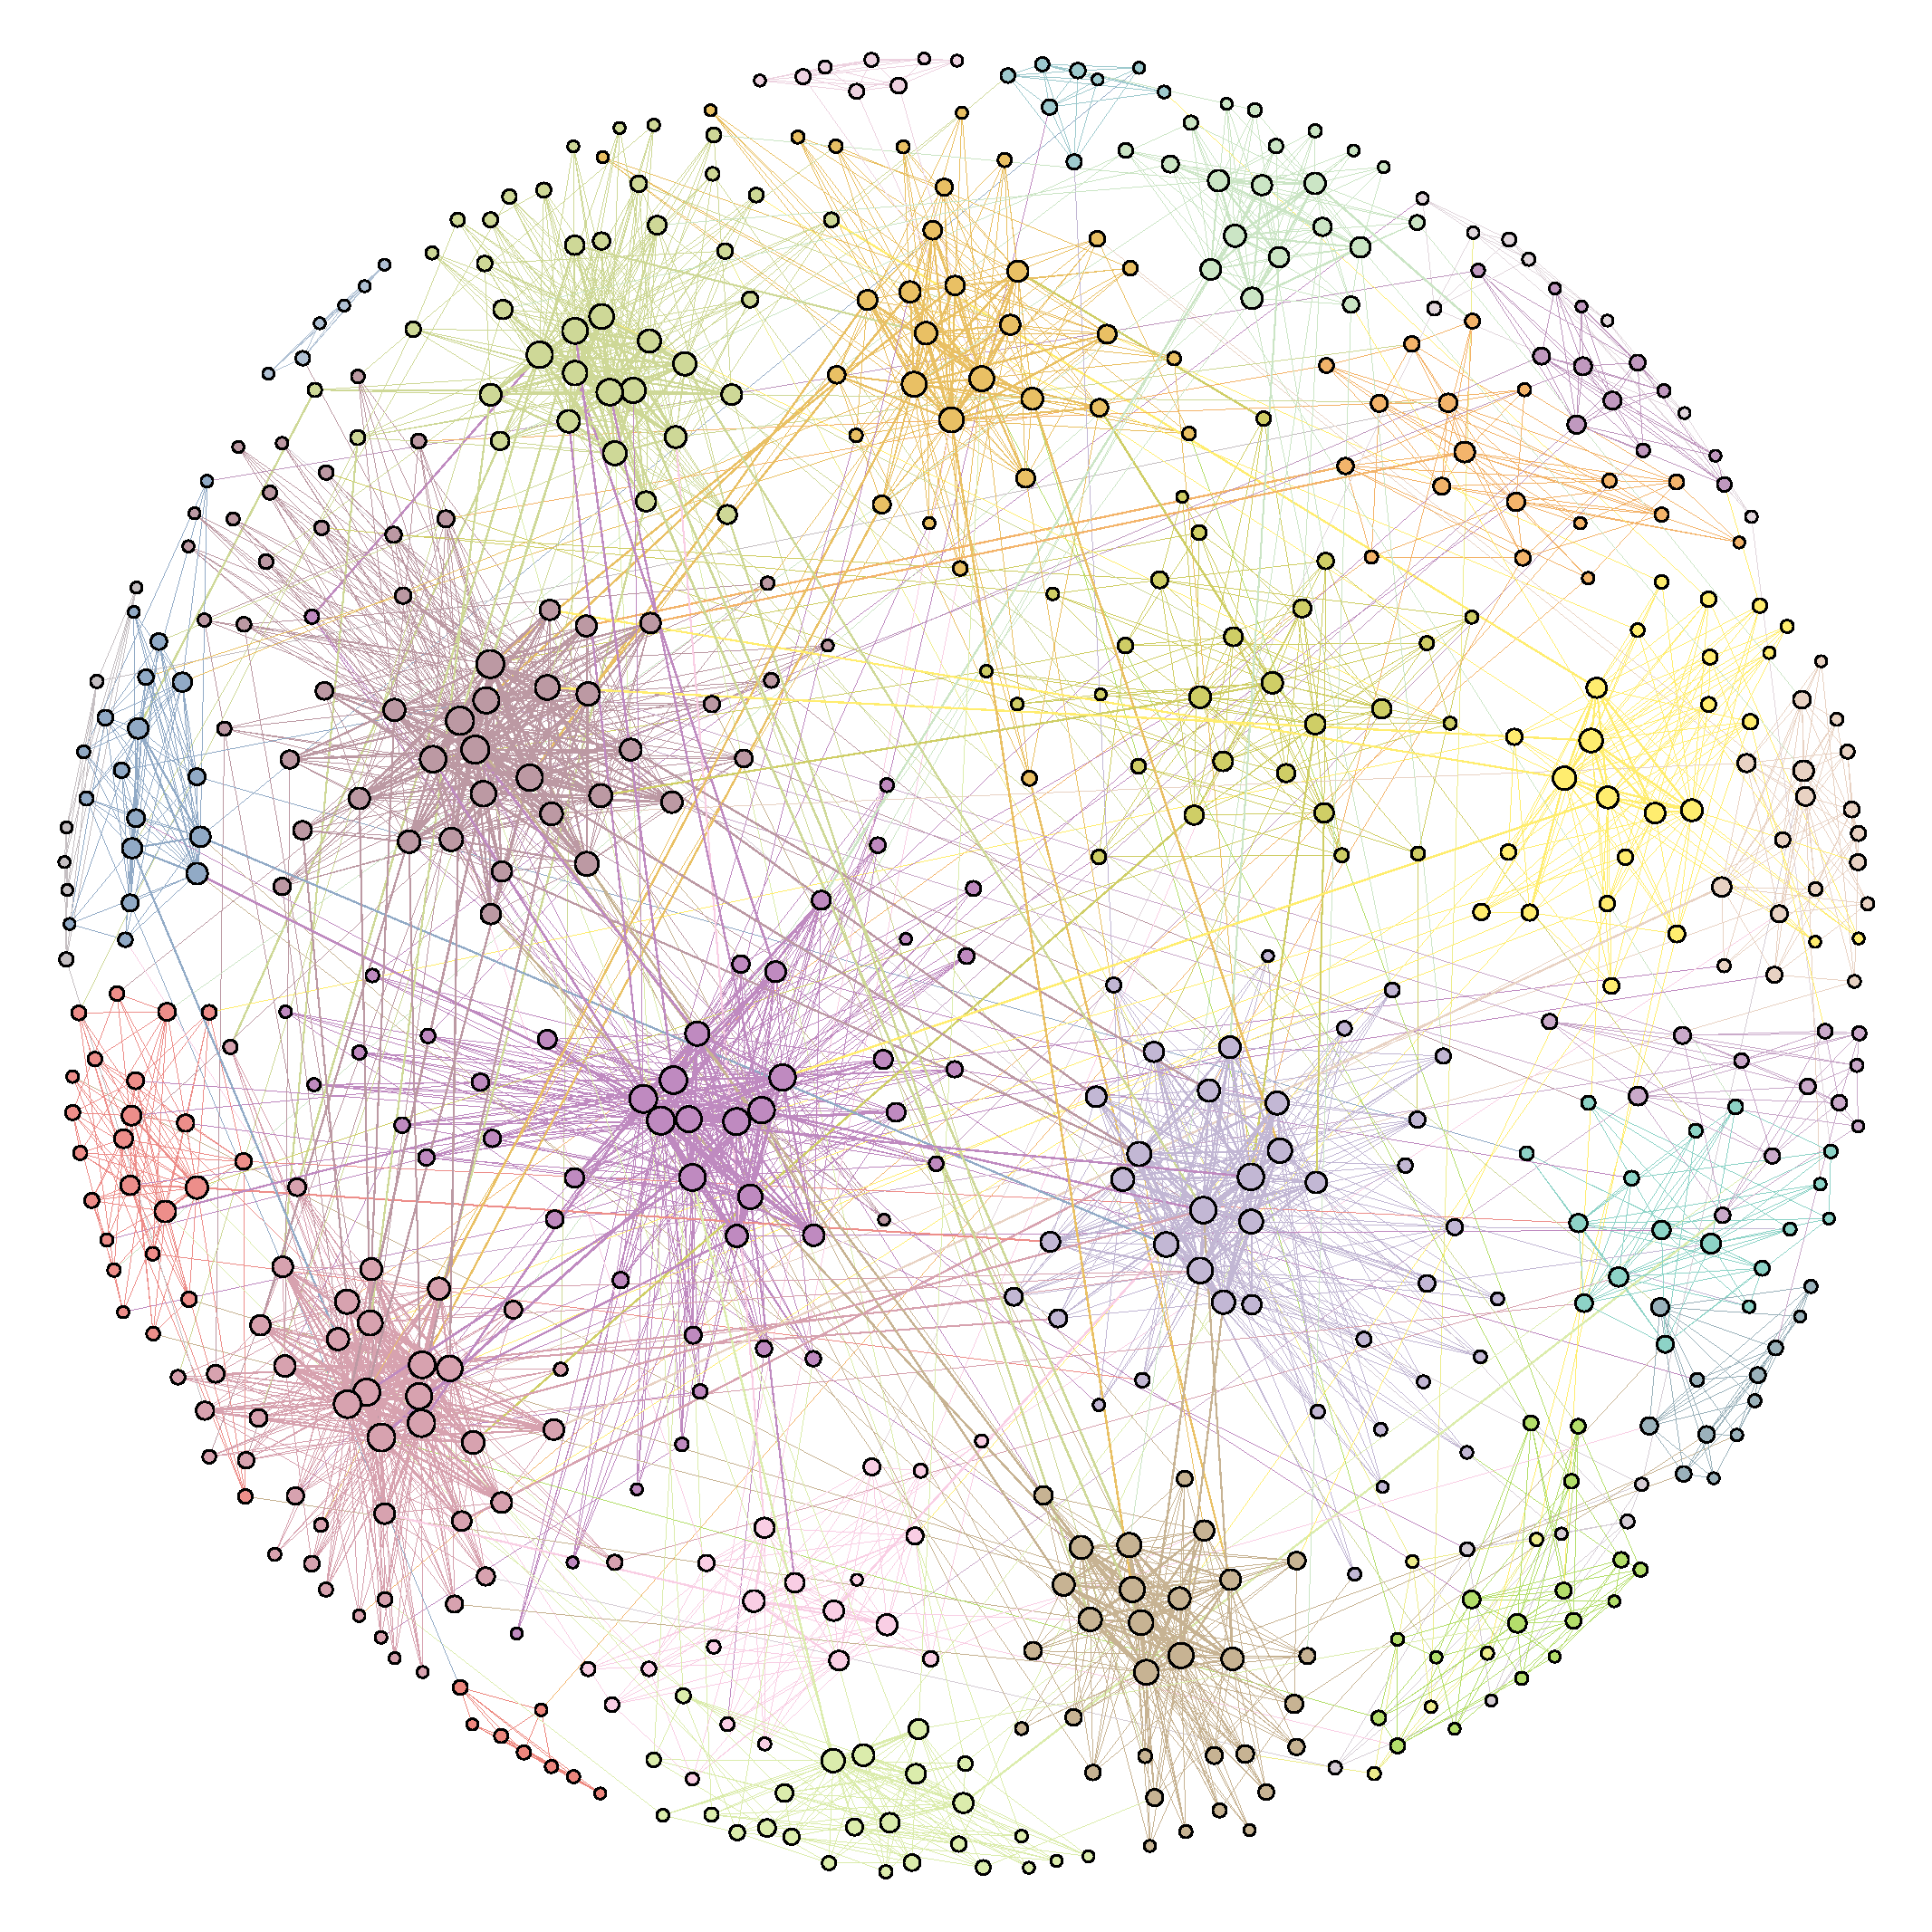
\includegraphics[width=1\textwidth]{images/LFRexample.pdf}
\end{minipage}
\end{footnotesize}
\caption{LFR parameters and a single instance with $n=600$, $\left<k \right>=12$, $\tau_d=2$, $\tau_c=1$, $\mu_t=0.1$, $\mu_w=0.1$, $\min_c=5$, $\max_c=50$.}
\label{tab:lfrparams}
\end{figure}

The LFR model is a great importance as it served as benchmark test for community detection algorithms and as model of heterogeneity of modules size when studying the performance of detection.

%%%%%%%%%%%%%%%%%%%%%%%%%%%%%%%%%%%%%%%%%%%%%%%%%%%%%%%%%%%%%%%%%%%%%
%%%%%%%%%%%%%%%%%%%%%%%% COMMUNITY DETECTION %%%%%%%%%%%%%%%%%%%%%%%%
\section{Community detection in networks}
\label{sec:communitydetectioninnetworks}
% Most of the real-world networks exhibit a degree distribution that is not only globally, but also locally inhomogeneous, with high concentrations of edges within special groups of nodes, and low concentrations among such groups. This feature of real networks is called community structure. 
The process of grouping nodes in a graph to establish their common behavioral properties, is a popular technique that goes under the name of \emph{community detection}.
As the definition of community is not well stated (section ~\ref{sec:communities}), it is therefore important to have a quantitative way to evaluate the goodness of such clusterings.

The previously introduced concept of global criterion for the definition of communities can be also thought in terms of a fitness function defined over the clustering.
A \emph{quality function} is a function $\mathcal{Q}$ that given a clustering of a graph $\zeta$ returns a scalar number. Usually one identifies ``good'' clusterings with high scores of the quality function and ``bad'' clusterings with low scores. In this sense, is possible to rank partitions from bad to good, although is important to stress that the definition of ``good'' or ``bad'' is an \emph{ill-posed problem} as every quality function one designs puts the emphasis on some features of the community organization and perhaps not on others. 
Here and in the following sections, we strongly stress that the concept of quality function and community detection methods are separate as the first is a way to assess the goodness of a partition while the second relies on the definition of a quality function to design efficient algorithms and heuristics to find such good partitions.

One of the most important properties of a quality function is when it can be expressed as a sum over communities. Such quality functions are dubbed \emph{additive}: for a generic function of a cluster, or subgraph, $f(\zeta_i)$, an additive quality function specify the goodness of a clustering as sum of $f$ over the distinct communities as follows:
\begin{equation}\label{eq:additive_quality}
\mathcal{Q} = \sum \limits_{\zeta_c \in \zeta} f(\zeta_c).
\end{equation}
The majority of quality functions are additive, even if this requirement is not fundamental. In the next section we explore the properties of some of the most important additive quality functions that emerged from the literature of this decade.

\subsection{Spin glass based quality functions}
The simplest requirement of a quality function, is to put emphasis on intracluster edges and penalize intercluster edges. In this terms, local optima should correspond to partitions where the communities emerge as dense areas in the network loosely connected among them.
Here we present a general framework for the definition of suitable quality functions for community detection that meets these requirements.

This framework, introduced by Reichardt and Bornholdt~\cite{reichardt2006} is grounded in statistical mechanics, a branch of physics that studies the macroscopic and microscopic properties of systems of many interacting elements. Within this model, the problem of community detection is cast in terms of finding the \emph{ground state} of a spin glass, a model describing the behavior of large sets of interacting microscopic magnets.
Actually, the properties of spin glass models are subject of extremely intensive research in the last decades as their applications range from matter and nuclear physics to neural networks. Here we present only their salient application to community detection and refer the reader to cover the details of the model in other specialized books~\cite{mezard1990}.

A spin glass model starts from the definition of an Hamiltonian, a multi-variable scalar function that describe the total energy of the physical system with the configuration of its internal components. In our case, the internal components of the system are the nodes. The configuration of the system is then expressed by the community affiliation vector $\boldsymbol\sigma$, meaning that node $i$ stays in the community $\sigma_i$ (see~\ref{sec:clustering}).
The Hamiltonian used by Reichardt and Bornholdt (RB) counts four different contributions. The first two contributions act at intracluster level, positively weighing intracluster edges and negatively weighing intracluster non-edges with coefficients $a_{ij}$ and $b_{ij}$ respectively. The third and fourth contributions work on intercluster edges and non-edges, weighing them with factors $c_{ij}$ and $d_{ij}$. The general form of the RB model is then expressed by the following Hamiltonian:
\begin{align}\label{eq:hamiltonianspinglass}
\mathcal{H}^{\textrm{RB}}(\boldsymbol \sigma) = - \sum_{(i,j)\in V^2} & \left[ a_{ij} A_{ij} - b_{ij}(1-A_{ij}) \right] \delta(\sigma_i,\sigma_j) + \nonumber \\ &  \left[ (c_{ij} A_{ij} - d_{ij}(1-A_{ij}) \right] (1-\delta(\sigma_i,\sigma_j))
\end{align}
with the convention that lowest energy states correspond to best community assignments.
Rearranging Eq.\ref{eq:hamiltonianspinglass} and discarding the terms independent of the partition into a constant $H_0$, one then gets a simpler expression for $\mathcal{H}^{\textrm{RB}}(\sigma)$:
\begin{equation}\label{eq:rbspinglass}
\mathcal{H}^{\textrm{RB}}(\boldsymbol \sigma) = -H_0 - \sum \limits_{(i,j)\in V^2} \left[ \alpha_{ij} A_{ij} - \beta_{ij} \right] \delta(\sigma_i,\sigma_j)
\end{equation}
where the two parameters $\alpha_{ij}=a_{ij}+b_{ij}+c_{ij}+d_{ij}$ and $\beta_{ij}=b_{ij}+d_{ij}$ depend on the \emph{null model} one would like to compare with, i.e. the probability that an edge exists between $i$ and $j$ after random edge rewiring. Hence, a null model provides a mean to compare a specific set of features of a graph, with its randomized version that should specifically lack those features.

It's possible to express any quality function in the form of Eq.~\ref{eq:rbspinglass} as an additive quality function by setting $\alpha_{ij}=1$, $H_0=0$ and moving the summation indexes over the communities rather than over the pairs of nodes, as the sum is only over intracluster edges. The resulting Hamiltonian, expressed here as $\mathcal{H}^{\textrm{RB}}_{\textrm{reduced}}(\sigma)$, then reads:
\begin{equation}\label{eq:rbspinglass2}
\mathcal{H}^{\textrm{RB}}_{\textrm{reduced}}(\sigma) = -\sum_{(i,j) \in V^2} \left[ A_{ij} - \beta_{ij} \right] \delta(\sigma_i,\sigma_j) = - \sum \limits_{c}^C \left[ m_c - \left< m_c \right> \right].
\end{equation}
where $m_c=\sum_{ij}A_{ij}\delta(\sigma_i,c)\delta(c,\sigma_j)$ represents the number of links inside community labeled by $c$ and $\left <m_c \right >=\sum_{ij}\beta_{ij}\delta(\sigma_i,c)\delta(c,\sigma_j)$ is the expected number of links in community $c$ as prescribed by the null model $\beta_{ij}$\footnote{Here and for the rest of the work, we set $P_{ij}:=\beta_{ij}$ for agreement with more conventional notation of null models}. 
Among the additive quality functions that show up in the form of~\ref{eq:rbspinglass2}, the most important and popular is the \emph{Newman-Girvan's Modularity}.

\subsection{Newman-Girvan Modularity}\label{sec:newman_modularity}
Newman-Girvan Modularity (or simply Modularity)~\cite{newman2006}, denoted here and for the rest of the work by $Q^N$, is based on the idea that a network obtained by randomly reshuffling the original graph edges while keeping the same degrees sequence, should not display any community structure. 
An important consequence of such randomization is that any stub in this null model, dubbed ``configuration model'' is equally likely to be connected to any other~\cite{newman2010networks}. Thus, in absence of correlations, the probability that two nodes are connected is expressed by:
\begin{equation}\label{eq:configuration_model}
P_{ij} = \frac{k_i k_j}{2m}
\end{equation}
where $k_i$ and $k_j$ are the degrees of node $i$ and $j$. The ``configuration model''  is of great importance in network science as it assigns higher probability of link to nodes with high degrees, a feature that is compatible with most real world networks. 
We'll address the motivations of the configuration model in  details in section~\ref{sec:configuration_model}.

In terms of a spin glass model, Modularity measures the deviation from the observed intracluster density with respect to the expected intracluster density specified by the configuration model. Modularity is described in the form of~\ref{eq:rbspinglass2} but normalized by the number of edges in the graph, taking the form described in Eq.~\ref{eq:newmanmodularityspinglass}.
\begin{equation}\label{eq:newmanmodularityspinglass}
Q^N =  \frac{1}{2m} \sum_{ (i,j) \in V^2} \left[ A_{ij} - \frac{k_i k_j}{2m} \right] \delta(\sigma_i,\sigma_j),
\end{equation}
whereby optimal partitions have high values of $Q^N$. As already done in Eq.~\ref{eq:rbspinglass2}, Modularity can alternatively be expressed, as sum over communities of the difference of two terms:
\begin{equation}\label{eq:newmanmodularity}
Q^N = \sum_{c}^{|C|} \left[ \frac{m_c}{m} - \left( \frac{K_{\textrm{int}}(\mathcal{G}_c)}{2m} \right)^2 \right]
\end{equation}

Modularity takes values in the range $[-0.5,1]$, then a good partition should have $Q^N$ values close to unity, identifying groups with many more internal connections than expected at random. In contrast, a bad partition with $Q^N$ closer to zero should identify groups with no more internal connections than we expect at random.
In the next sections we will challenge this idea and show that this observation has lead to false statements, as a general phenomenon dubbed \emph{resolution limit}, heavily affects any quality function based on comparison with global null models. Specifically in the case of Newman's Modularity, the resolution limit hit hard.

\subsection{The configuration model}\label{sec:configuration_model}
A central property of the configuration model is the probability $P_{ij}$ of the occurrence of an edge between two specified vertices $i$ and $j$.
Let's consider anyone of the stubs that emerges from vertex $i$.
What is the probability that this stub is connected by an edge to any of the stubs of vertex $j$?
There are $2m$ stubs in total, or $2m - 1$ excluding the one connected to $i$ that we are currently looking at.
Of those $2m - 1$, exactly $k_j$ of them are attached to vertex $j$.
So, given that any stub in the network is equally likely to be connected to any other, the probability that our particular stub is connected to any of those around vertex $j$ is $k_j/(2m-1)$.
In absence of correlations, the probabilities that any two nodes $i$ and $j$ are connected to each other is given by the sum of the two independent probabilities for vertex $i$ and vertex $j$, defining the null model as:
\begin{equation}\label{eq:configuration_model_probability}
P_{ij} = \Pr \left ( a_{ij} | \{ k \} \right) = \Pr(k_i | \{ k \}) + \Pr(k_j | \{ k \})=\frac{k_i k_j}{2m}
\end{equation}

Although Modularity is most frequently applied to \emph{simple graphs} (see Fig.~\ref{fig:simple_unweighted_graph}), the configuration model implies that the randomization is carried over the space of \emph{loopy multigraphs} (Figure~\ref{fig:loopy_multigraph}).
The rewiring probability considers indeed that the stubs of nodes can be reconnected both to the same source vertex (self-loops) or added to already existing edges (multi-edges).
Consider for example the set of matchings on six stubs that form a triangle graph as illustrated in Figure~\ref{fig:configuration_model_stubs}. The configuration model chooses each distinct edge stubs labeling with equal probability. However, not only the first eight distinct reshuffled labellings are possible under configuration model (Fig.\ref{fig:reshuffle_simple_graphs}) but many other distinct matchings producing non-simple networks as shown in Figure~\ref{fig:reshuffle_loopy_multigraphs}.
In fact, the number of possible re-wirings that can be generated under the hypotheses of the configuration model, namely the presence of self-loops and multi-edges, is indicated by $\Omega_{CM}$ and can be computed by means of combinatorial arguments as:
\begin{equation}\label{eq:cm_possible_rewirings}
\Omega_{CM} = \binom{2m}{k_1,\ldots,k_n} = \frac{(2m)!}{\prod_i^n k_i!}.
\end{equation}
For the small triangle graph, this number is already very large: 90 different re-wirings are possible!
In practice though, the fraction of edges involved in either self-loops or multi-edges is vanishingly small in the large $n$ limit, and thus we may generally ignore them without much impact. 
Hence, the estimate of the probability of rewiring in Eq.~\ref{eq:configuration_model_probability} is only valid in large, sufficiently sparse graphs with a sufficiently bounded degree sequence.
Under these hypotheses the expected number of edges between two vertices in the space of simple graphs is asymptotically the same as the expectation in the space of stub-labeled loopy multigraphs, i.e. the one previously introduced for the definition of Modularity: $\mathbb{E}_s[a_{ij} |k] \approx k_i k_j /(2m)$, where the subscript $s$ denotes the space of simple graphs.

\begin{figure}[htb]\centering
\begin{subfigure}[t]{0.45\textwidth}\centering
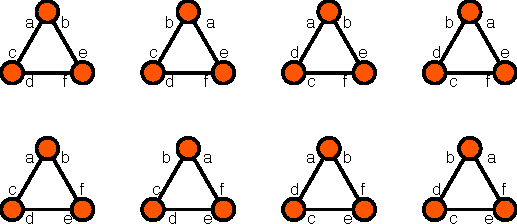
\includegraphics[height=2.4cm]{images/configuration_model_six_stubs.pdf}
\caption{}
\label{fig:reshuffle_simple_graphs}
\end{subfigure}
\begin{subfigure}[t]{0.45\textwidth}\centering
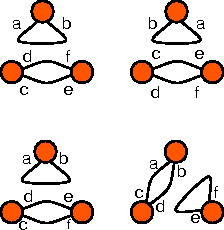
\includegraphics[height=2.4cm]{images/configuration_model_three_stubs.pdf}
\caption{}
\label{fig:reshuffle_loopy_multigraphs}
\end{subfigure}
\caption{Twelve of the ninety different possible rewirings of a triangle graph in the configuration model. In (a) only rewirings leading to simple graphs are considered. In (b) just four rewirings leading to loopy-multigraphs are shown.}
\label{fig:configuration_model_stubs}
\end{figure}
An approach that allows to get the right configuration model depending on the class of graph under exam, relies on the computational simulation of the correct rewiring probability by means of Markov Chain Monte Carlo algorithms, as proposed in~\cite{fosdick2016}.
In the remaining paragraphs, although flawed, we'll use the classic configuration model from Eq.~\ref{eq:configuration_model_probability} to be adherent to most of the brain networks literature, justified also by the vanishing effects of self-loops in large sparse networks. Nonetheless, we will illustrate many of the problems that the non critical use of Modularity with this null model has introduced.

\subsection{Other null models for Modularity}
Modularity identifies communities as subset of nodes whose internal fraction of edges deviates from the null configuration model on the same subset with the term $m_c/m > (K_c/2m)^2$.
Despite measuring deviation from a null model, Modularity does not take into account the statistical evidence associated with this deviation. For this reason, Modularity is not able to separate actual communities from those arising only from statistical fluctuations of the null model. Even worse, Modularity can find high-scoring partitions in fully random graphs~\cite{guimera2004} and in artificially built graphs with no community structure~\cite{kehagias2013}.

The configuration model is not the only possible null-model to use in spin-glass based quality functions. Different authors proposed several variants of Modularity~\cite{ronhovde2010,ronhovde2009,traag2011} with different null models.
The simplest variation of Modularity is the so-called ER Modularity~\cite{traag2015} that instead of the configuration model uses an Erd\H{o}s-Rényi random graph in which every edge appears with the same probability $p_{\textrm{ER}}$. The number of expected edges $\left< m_c \right>$ in a community of size $n_c$ is thus (in the space of simple graphs):
\begin{equation}
\left< m_c \right> = p_{\textrm{ER}}\binom{n_c}{2}.
\end{equation}
and plugging this null model into the RB model of Eq.~\ref{eq:rbspinglass2} we obtain the model:
\begin{equation}\label{eq:ermodularityrb}
\mathcal{H}^{ER} = -\sum \limits_c^C \left[\frac{m_c}{m}  - p_{\textrm{ER}}\binom{n_c}{2} \right].
\end{equation}
As the most similar ER graph of a given graph is the one that matches its density, the probability parameter $p_{\textrm{ER}}$ must be set equal to the original empirical graph density $\rho$. The so-called ER Modularity is derived by plugging the graph density in Eq.\ref{eq:ermodularityrb} and inverting its sign: 
\begin{equation}
Q^{ER} = \sum \limits_c^C \left[\frac{m_c}{m}  - \rho \binom{n_c}{2} \right].
\end{equation}
Under this model a group of nodes forms a community if its internal density is greater than the graph density $\rho$, on average.
Interestingly, from a machine learning perspective, all spin glass models quantify the discrepancy between observed and expected intramodule fraction of edges by means of a linear loss function. Among all the loss function, the linear is not the only possible and loss functions that take into account the relative size of clusters are possible.

\subsection{Comparing community structure in networks}
Some benchmark networks come with an annotated community structure representing the ground-truth assignment of nodes into communities, the annotations being made by experts in the field, like for example the karate-club network of Zachary~\cite{zachary1977} or the political blog network~\cite{adamic2005}.
Moreover, generative models of networks like the stochastic block model and its variants, the planted partition model and the LFR benchmark, have a known ground-truth community.
As the number of community detection methods increased over the years, also a quantitative way to assess their performance was requested.

A large number of functions for comparing similarities and differences between partitions of a network have been proposed in the past. They are used to provide quantitatively a number that tells how two partitions are similar.
Typically the result is normalized in the $[0,1]$ range, being towards $1$ for very similar clusterings and toward $0$ when mostly dissimilar. These metrics are adopted especially in the benchmarking of community detection methods, when the specific outcome of some algorithm is compared with a ground truth partition, usually a-priori determined.

The most well-grounded and performing metrics for the comparison of two community structures are rooted in information theory\cite{cover2006}.
The \emph{Normalized Mutual Information}~\cite{danon2005} and the \emph{Variation of Information}~\cite{meila2007} are the most widely used, despite it has been recently found that both of them suffer of systematic errors due to the finite size of the network \cite{zhang2015a}. In the rest of the discussions we ignore the limitation of finite size effects, by only working with relatively large networks.

Normalized Mutual Information (NMI) assumes that the clustering comparison is a problem of message decoding. Implicit in this, is the idea that if two partitions are similar, inferring one partition from the other needs very little information. 

Let us consider two generic partitions of a graph denoted by their clusterings $\zeta^x,\zeta^y$ with $c_x$ and $c_y$ communities respectively: $\zeta^x=\{\zeta^x_1,\ldots,\zeta^x_{c_x}\}$ and $\zeta^y=\{\zeta^y_1,\ldots,\zeta^y_{c_y}\}$.
The number of nodes in the $i$-th community of $\zeta^x$ is $n_i :=|\zeta^x_i|$ and the number of nodes in the $j$-th community of $\zeta^y$ is $n_j:=|\zeta^y_j|$. The two communities share a number of nodes $n_{ij}=| \zeta^x_i \cap \zeta^y_j|$.
Let us also consider the community assignments $\boldsymbol\sigma^x_i$ and $\boldsymbol\sigma^y_i$ for partitions $\zeta^x$ and $\zeta^y$ respectively; we treat the labels as values of two random variables $X$ and $Y$ with joint distribution $P(x,y)=P(X=x, Y=y) = n_{xy}/n$, which implies that $P(x)=P(X=x)=n_x^X/n$ and $P(y)=P(Y=y)=n_y^Y/n$.
The \emph{mutual information} between the two clusterings $\zeta^x,\zeta^y$ is then defined as 
\begin{equation}I(X,Y)=H(X) - H(X|Y)
\end{equation}
where $H(X)=-\sum_x p(x) \log p(x)$ is the Shannon entropy of $X$~\cite{cover2006}.
The mutual information itself is not very useful, because hierarchically splitting the clusters in $\zeta^x$ would produce no change in the prior $H(X|Y)$ and partitions with different hierarchies of the same clusters, would go unnoticed.
This observation led Danon~\cite{danon2005} to introduce normalized mutual information for clustering comparison as: 
\begin{equation}\label{eq:nmi}
\textrm{NMI}(X,Y) = \frac{2I(X,Y)}{H(X)+H(Y)}
\end{equation}
Explicitly, NMI is defined on top of the confusion matrix as:
\begin{equation}\label{eq:nmiexplicit}
\textrm{NMI} = \dfrac{2\sum \limits_{i=1}^{c_x} \sum \limits_{j=1}^{c_y} \frac{n_{ij}}{n} \log\left( \frac{n_{ij}n}{n_i n_j} \right)} {\left(-\sum \limits_{k=1}^{c_x} \frac{n_k}{n}\log\left(\frac{n_k}{n}\right) \right) + \left(-\sum \limits_{k=1}^{c_y} \frac{n_k}{n}\log\left(\frac{n_k}{n}\right) \right)}
\end{equation}

\begin{figure}
\centering
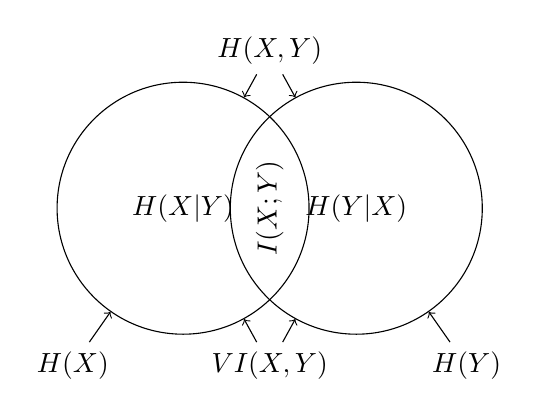
\begin{tikzpicture}
    \node[draw,circle,minimum size=3.2cm, inner sep=0cm] at (-1.1cm,0cm) (CL) {$H(X|Y)$};
    \node[draw,circle,minimum size=3.2cm, inner sep=0cm] at (1.1cm,0cm) (CR) {$H(Y|X)$};    
    \node[rotate=90] at (0cm,0cm) (IXY) {$I(X;Y)$};
    \node[] at (0cm,2cm) (HXY) {$H(X,Y)$};
    \node[] at (-2.5cm,-2cm) (HX) {$H(X)$};
    \node[] at (2.5cm,-2cm) (HY) {$H(Y)$};
    \node[] at (0cm,-2cm) (VI) {$VI(X,Y)$};
    \draw[->] (HX) -- (CL);
    \draw[->] (HY) -- (CR);
    \draw[->] (HXY) -- (CL);
    \draw[->] (HXY) -- (CR);
    \draw[->] (VI) -- (CL);
    \draw[->] (VI) -- (CR);
\end{tikzpicture}
\caption{Venn diagram representation of the important quantities used to treat the clustering comparison problem in terms of information theory. The two circles are the entropies of variables $X$ and $Y$. The mutual information $H(X;Y)$ is the intersection of the information in $X$ with the information in $Y$. The Variation of information is equal to $VI(X;Y)=H(X|Y)+H(Y|X)=H(X)+H(Y)-2I(X;Y)$ because $I(X;Y)$ is counted twice.}
\end{figure}

Meila proposed another measure based on entropy, Variation of Information (VI)~\cite{meila2007}. VI measures how much knowing the cluster assignment for an item in clustering $X$ reduces the uncertainty about the item's cluster in clustering $Y$. Is defined as:
\begin{equation}\label{eq:vi}
\textrm{VI}(X,Y) = H(X|Y) + H(Y|X)
\end{equation}
and it has the desirable property that, being a proper distance, it defines a metric on the space of the partitions.
Variation of information is also a local measure, i. e. the similarity of partitions differing only in a small portion of a graph depends on the differences of the clusters in that region, and not on the partition of the rest of the graph.
As noted by Karrer \cite{karrer2008} VI is upper-bounded by a $\log(n)$ factor, so a simple normalization brings it in the $[0,1]$ range. 
Importantly, VI is zero for maximally equal partitions and $1$ for mostly dissimilar, inversely to NMI.

It's worth noting that the majority of the aforementioned metrics do not take in consideration comparison of pairs of communities between two partitions, but they insist on finding overall similarity to summarize it in a single scalar.

% It is possible though to study partitioning on a community-wise basis by explicitly enumerating all the similarity between groups of nodes of two different partitions.

% Let's assume we have two different clusterings $\zeta^x,\zeta^y$ obtained from two different runs of some non-deterministic community detection algorithm. For two communities $c_i \in \zeta_1, c_j \in \zeta_2$, with $1\leq i \leq |\zeta_1|$,$1\leq j \leq |\zeta_2|$ then the cluster homogeneity is defined as:

% \begin{align}
% \Pr(\textrm{overlap}) = \frac{\binom{|c_j|}{|c_i \cap c_j|}\binom{N-|c_j|}{|c_i|-|c_i \cap c_j|}}{\binom{N}{|c_i|}}
% \end{align}
% %
% \todo{fix discorso cluster homogeneity}

\section{Resolution limit}\label{sec:resolutionlimit}
Modularity attracted a lot of attention over the years as it  became the tool of election to inspect the community structure of networks.
On one side, the wide use of Modularity, led many researchers to gain interest in complex networks, with results in sociology~\cite{li2008tag}, bioinformatics~\cite{saracc2012topology} and ICT~\cite{java2007we,leskovec2007dynamics}, just to mention a few, but on the other side it offered a fallacious view on the community detection problem.
Indeed, although simple in many sense, Modularity optimization was hiding a problem that heavily limits its use in real world networks.

In 2007, a seminal article by Fortunato and Barthelemy~\cite{fortunato2007} did a thoroughly analysis of Modularity.
Their work showed the inability of Modularity to correctly identify communities that are smaller than a certain scale, determined by the square root of the number of edges. They dubbed this general phenomenon \emph{resolution limit}.
To illustrate what is meant by the resolution limit, here we follow the example of Fortunato and Barthelemy, with some obvious notational change.

Let us consider a toy network, $G=(V,E)$ that is composed of three subnetworks, as shown in~\ref{fig:figure_1_barthelemy}A.
The first subnetwork, a subgraph $G_0$ with $n_0$ nodes and $m_0$ edges is connected to two cliques, $G_1$ and $G_2$ by $m_{01}$ and $m_{02}$ links respectively. The two cliques are also connected by a number of $m_{12}$ links as shown in Figure~\ref{fig:figure_1_barthelemy}.
While $G_1$ and $G_2$, are complete subgraphs and are expected to be modules by construction, $G_0$ may consist of many communities. Maximum Modularity partitions then, should identify $G_1$ and $G_2$ as communities, independently from $G_0$.
To be more specific, let the partition where the two cliques are separated be denoted by $A$, with Modularity value $Q_A$. On the other hand, the partition where the two cliques are merged into a single community is denoted by $B$, with Modularity value $Q_B$.
To ease the calculations, we indicate the number of links $m_{12}$ as functions of $m_1$ and $m_2$, such that $m_{12}=a_{1}$, $m_1=a_2 m_2$, $m_{01}=b_1 m_1$ and $m_{02}=b_2 m_2$ with $a_1,a_2,b_1,b_2 \geq 0$.

As Modularity is a sum over the modules, and the module $G_0$ has the same Modularity $Q_0$ in both partitions, we are interested in studying the difference $\Delta Q = Q_{A} - Q_{B}$. After some simple algebraic manipulations it results:
\begin{equation} \label{eq:resolution_limit_delta}
\Delta Q = \frac{2 m a_1 m_1 - (a_1+b_1+2)(a_2+b_2+2)m_1 m_2}{2m^2}
\end{equation}
Specifically, we want to check when $\Delta Q > 0$, i.e. when the partition $A$ has a higher Modularity than partition $B$. This condition is verified as long as
\begin{equation}
m_2 < \frac{2m a_1}{(a_1+b_1+2)(a_2+b_2+2)}.
\end{equation}
In the case where $a_1=a_2=0$, there are no links between $G_1$ and $G_2$ and the condition is satisfied. When instead the two subgraphs are connected ($m_{12} \neq 0$), it happens that at some values of $m_1$ and $m_2$, the partition where the two modules are merged is preferred, i.e. $\Delta Q <0$. This means that when maximizing $Q^N$ on a network, is possible to miss some important structures, if they are too small.
More specifically, if the two modules have the same size and one sets $a_1=a_2=b_1=b_2=1/m$, is easy to check that Eq.~\ref{eq:resolution_limit_delta} is not satisfied if the number of links in the modules $m_c$, is lower than the square root of the total number of links in the network:
\begin{equation}
m_c < \sqrt{\frac{m}{2}}.
\end{equation}

To make this example more concrete we studied numerically a toy network where the three subgraphs take a precise form.
For the sake of illustration, we have defined $G_1$ and $G_2$ as two identical cliques of $5$ nodes connected to $G_0$ by a single edge ($m_{01}=m_{02}=1$) and to each other by $m_{12}$ edges.
The module $G_0$ was defined as a clique of variable size with a number of edges ranging from 45 to 2775. We then computed the numerical difference $\Delta Q$ and plotted it as a function of the number of edges $m_0$ in the $G_0$ clique. The onset of the resolution limit occurs when $\Delta Q$ changes sign and becomes negative for increasing values of $m_0$.
For $m_{12}=1$, i.e. when the two cliques $G_1$ ad $G_2$ were connected by only one edge (red curve), $Q$ showed this sign inversion for $m_0 \approx 200$ (Figure \ref{fig:figure_1_barthelemy}B).
With increasing number of intercluster edges $m_{12}$, the resolution limit appeared for smaller and smaller values of $m_0$, eventually leading to $\Delta Q$ values that were always negative, i.e. the two cliques $G_1$ and $G_2$ were always merged by Modularity optimization.


\begin{figure}[htb!]
\centering
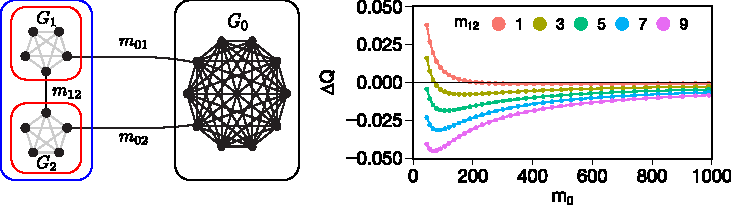
\includegraphics[width=1\textwidth]{images/barthelemy_modularity.pdf}
\caption{Analysis of the onset of the resolution limit for Modularity in a model graph (A) consisting of two cliques, $G_1$ and $G_2$, and a size-varying components $G_0$. The red line indicates the partition $A$, with $G_1$ and $G_2$ as different modules, and the blue line the partition $B$, with $G_1$ and $G_2$ merged into a single module. The graph (B) shows the difference in Modularity for increasing number of edges in $G_0$.}
\label{fig:figure_1_barthelemy}
\end{figure}

An even more striking example of how the resolution limit affects Modularity is when looking at the optimal partition of a synthetic lattice graph, known as ``ring of cliques'', a network made out of identical cliques, connected in a ring-like structure by single links, as shown in Figure~\ref{fig:traag_ring_of_cliques}. 

\begin{figure}[htb!]
\centering
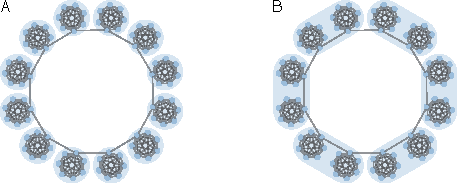
\includegraphics[width=1\textwidth]{images/traag_ring_of_cliques.pdf}
\caption{In this toy network, the intracommunity density is the highest possible, while the intercommunity density is the lowest to keep the network connected. The correct community structure is clearly the one on left (A), but Modularity values is higher for the partition on the right (B), where pairs of cliques are coalesced into separated communities.}
\label{fig:traag_ring_of_cliques}
\end{figure}
If the number of cliques is large enough (they are more than $\sqrt{m}$), Modularity optimization leads to a partition where the cliques are combined into groups of two or more. This phenomenon can be observed already when considering a ring of 30 cliques made of 5 nodes, when the optimal Modularity partition combines cliques in pairs.
Yet extending the number of cliques, Modularity may merge cliques into groups of three, fours etc.

\subsection{Resolution parameter}
Fixes have been proposed to circumvent the resolution limit, including the introduction of a tunable parameter that enables analysis of the network at an adjustable resolution level~\cite{reichardt2006,ronhovde2010,yeo2011}.

In this sense, the most common tuning to the Modularity quality function is the one that takes in consideration a \emph{resolution parameter}.
From the definition of $Q^N$ is evident that is possible to tune the size of the detected modules by multiplication of the configuration null model by a constant factor $\gamma_{N} \in [0,1]$, resulting in a modified modularity $Q^N(\gamma)$:
\begin{equation}
Q^N(\sigma,\gamma) = \sum_c^C \left[ \frac{m_c}{m} - \gamma_{N} \left( \frac{K_c}{2m}\right)^2 \right].
\end{equation}
However, exact specification of $\gamma_{N}$ requires prior knowledge of the expected size of the communities.
Moreover, it has been shown~\cite{lancichinetti2011} that an adjustable resolution parameter may reduce the tendency to merge small clusters, but only at the cost of unduly splitting large clusters. 
Indeed this is due to two opposite coexisting effects: the tendency to merge small subgraphs, which dominates when the resolution is low and the tendency to split large subgraphs, which dominates when the resolution is high.

In benchmark networks with heterogeneous distributions of cluster sizes, the simultaneous elimination of both biases is not possible and multi-resolution modularity is not capable to recover the planted community structure even in graphs where the ground-truth structure is evident.
Therefore, adjustment of the resolution parameter is an attempt to balance these two biases, but multi-resolution methods fail to recover community structures comprising heterogeneous distributions of cluster sizes~\cite{lancichinetti2011}. 

In another attempt to better tolerate the resolution limit, scholars applied appropriate techniques of edge re-weighting~\cite{berry2011} to enhance communities prior to Modularity maximization.
Although this technique proved able to better tolerate the detrimental effect of the resolution limit, it only shifted the scale of the problem.
After all, real-world networks are characterized by the coexistence of clusters of very different sizes, therefore no single parameter can adapt to the variety of network topologies observed in nature.

\subsection{Resolution-limit free quality functions and the Constant Potts Model}
In an attempt to quantitatively characterize the resolution limit, Traag et al.~\cite{traag2011} proposed a rigorous definition of \emph{resolution-limit-free} graph partitioning.

A quality function is resolution-limit-free if, given an optimal partition $\zeta$ of a graph $G$, any module $\zeta_i$ is also optimal for the graph induced by the nodes in $\zeta_i$.
In other words, each community of the optimal partition is not split by optimization of the quality function applied to the subgraph induced by the nodes in the community.
Hence, each community does not depend on the rest of the network and is both locally and globally optimal.
Then, in order to design such resolution-limit-free quality function, Traag took a spin glass model, with a null model specified by constant quantity $\gamma_{\textrm{CPM}}$~\cite{traag2011} and dubbed it \emph{Constant Potts Model}.

The \emph{Constant Potts Model} (CPM) identifies community as subset of nodes whose internal density $\rho_c$ is bigger than the overall graph density multiplied by a factor $\gamma_{\textrm{CPM}}$ that defines the typical scale of the communities. In the framework of Reichardt and Bornholdt, the CPM model has the following Hamiltonian: 
\begin{equation}\label{eq:cpm_hamiltonian}
H(\sigma)^{\textrm{CPM}} = - \sum \limits_{(i,j) \in V^2} \left[ a_{ij} - \rho \gamma_{\textrm{CPM}} \right] \delta(\sigma_i,\sigma_j),
\end{equation}
that once reworked in an additive quality function, results in the form of Eq.~\ref{eq:cpm_hamiltonian} 
\begin{equation}\label{eq:cpm_ermodel}
Q^{\textrm{CPM}} = \sum \limits_c^{|C|} \left[m_c - \gamma_{\textrm{CPM}} n_c^2 \right] 
\end{equation}
In other words, the model tries to maximize the number of internal edges while at the same time keeping relatively small communities. The parameter $\gamma_{\textrm{CPM}}$ balances these two imperatives; indeed it acts as the inner and outer edge density threshold.
In the CPM settings is better to split two communities $r$ and $s$ if $\gamma_{CPM}$ exceeds the inter-community density $m_{r,s}/(2n_r n_s)$.

Unfortunately, the operation of tuning the resolution parameter, both in the CPM model as well as in other similar models, is difficult and no largely accepted method exists, making all the models based on a resolution parameter, scarcely used in practical applications.

\subsection{Effects of resolution limit}
In the context of brain networks, the resolution limit first highlighted by Fortunato and Barthelemy may be particularly critical for the analysis of brain connectivity networks, as it may unduly merge modules that are too small, therefore hampering the ability to highlight regions of functional segregation from the rest.
By way of example, certain functional processes, like color vision, have been described as anatomically localized~\cite{zeki1998}, while others, like working memory, have been proposed to involve more globally integrated processing systems~\cite{baddeley2003}.

Hence, we may expect the brain modular structure to comprise heterogeneously distributed communities. Whether the relatively uniform modular structure of brain connectivity, highlighted by Newman's Modularity and other community detection methods in many studies, reflects the true architecture of the brain organization or is the result of the resolution limit is still unclear.
Hierarchical approaches have shown that large modules can be further subdivided, indicating that connectivity networks show structure at different spatial scales~\cite{meunier2009}.
However, these findings do not provide information on the optimal partition of the network, i.e. the optimal cut through the dendrogram representing connectivity at the different scales.

Thus, the resolution limit is a critical shortcoming for the study of brain networks and is likely to have affected many of the studies reported in the literature. The limitation on the number of detected modules in brain networks is evident in studies where typically four or five communities of the same size are detected in humans, as in Crossley et al.~\cite{crossley2013a}, Meunier et al.~\cite{meunier2009a,meunier2010}, Fair et al.~\cite{fair2009} or also in mouse models~\cite{schwarz2008}. To this end, an optimization method that does not suffer from the resolution limit would be needed.

It's also very important to stress that comparing the Modularity value $Q^N$ across different networks obtained in different studies, with possibly different number of nodes or different densities is an erroneous practice although $Q^N$ is normalized in the range $[0,1]$. As shown by a number of studies~\cite{good2009,kehagias2013,radicchi2010}, even in graphs which do have a natural community structure, high modularity values can be achieved by partitions which do not respect this natural structure. Hence, the Modularity value is only a numerical indication of the current status of optimization of the detected community structure on a specific graph and should never be confronted across different networks.


%%%%%%%%%%%%%%%%%%%%%%%%%%%%%%%%%%%%%%%%%%%%%
%%%%%%%%%%%%%% DEGENERACY %%%%%%%%%%%%%%%%%%%
%%%%%%%%%%%%%%%%%%%%%%%%%%%%%%%%%%%%%%%%%%%%%
\section{Degeneracy}\label{sec:degeneracy}
The differences in Modularity between optimal and suboptimal partitions can be very small, as observed in Figure~\ref{fig:figure_1_barthelemy}B, where $\Delta Q$ between the two partitions with splitted or merged cliques, remains close to zero for a large range of $m_0$ especially at $m_{12}=1$.
Indeed, even in the case where it would not be beneficial for Modularity to merge two modules, i.e $\Delta Q <0$, this difference can be made arbitrarily close to zero.

The total number of different partitions in a graph is the Bell number $B_n$~\cite{stanley1997} and it grows faster than exponentially in $n$, therefore a combinatorially large number of sub-optimal partitions exist around the global optimum. These partitions may be very close in terms of Modularity to the optimum but radically different in terms of similarity.
Thus, counter-intuitively, when the network becomes more modular, the globally optimal partitions becomes harder to find among the growing number of suboptimal but competitive alternatives.

This consideration explains the empirical observation that nearly-optimal solution tend to group into high-modularity plateaus, although they may differ substantially~\cite{good2009}. This phenomenon, dubbed \emph{degeneracy} affects Newman's Modularity and probably many other spin-glass based quality functions.
As a matter of example, the variation in Modularity for merging a pair of adjacent cliques in the ring of cliques graph shown in Figure~\ref{fig:traag_ring_of_cliques}, is given by:
\begin{equation}\label{eq:modularity_difference_ring_clique}
\Delta Q = \frac{1}{r\left(\binom{n_r}{2}+1\right)}-2r^{-2}
\end{equation}
where $r$ is the number of cliques and $n_r$ the number of nodes in each clique.
In the large $r$ limit, the difference in Eq.~\ref{eq:modularity_difference_ring_clique} tends to a small negative value, indicating that a solution where the cliques are merged, may have a Modularity very close to the optimum. Indeed, already for $r=20$ cliques, $\Delta Q \approx 5\times 10^{-3}$, making all the suboptimal partitions where cliques are merged, very close to the optimal solution.

To make this argument more intuitive, we extrapolated a visually appealing form of the complex landscape of partitions' Modularity for a ring of clique network. We sampled the configuration space of the partitions of a ring of clique network through a Montecarlo procedure and annotated the corresponding values of Modularity for every partition.
We then built a similarity matrix between all sampled partitions and embedded it into a three-dimensional space maintaining similarity relations between partition following a Curvilinear Components Analysis (CCA).
In the embedded manifold, two partitions are close if they are similar and the z-axis encodes the quality function.
An highly degenerate plateu can be observed in~\ref{fig:degeneracylandscape} whereby different solutions with high values of Modularity stay in the same neighborhood.

\begin{figure}[htb!]
\centering
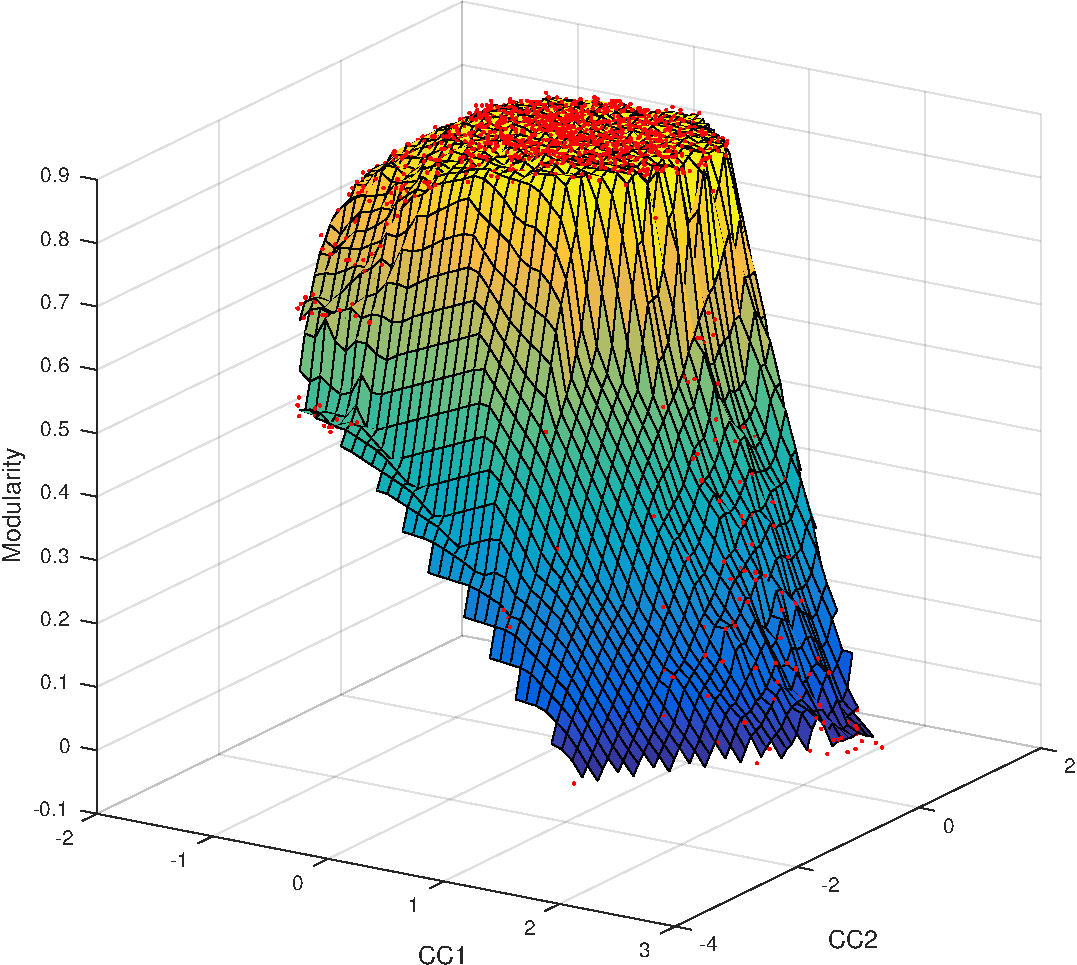
\includegraphics[width=0.6\textwidth]{images/degeneracy_modularity.pdf}
\caption{Degeneracy landscape for Newman's Modularity in a ring of cliques with $r=24$ cliques of $n_r=5$ nodes. The axes CC1 and CC2 are complicated functions of the original partition space computed as to maintain the distance relation between points and their scale is unimportant.}
\label{fig:degeneracylandscape}
\end{figure}

Any quality function suffering degeneracy of solutions, should display an embedded landscape with a plateau of optimal partitions, like the one shown in Figure~\ref{fig:degeneracylandscape}, while instead in the case of the existence of a net global optimum, a sharper peak should be exhibited.
We'll see that recasting the problem of community detection in terms of probability theory, will help in the definition of a quality function showing convex behavior and uniqueness of the optimum solution.